%%
%% This is file `sample-acmtog.tex',
%% generated with the docstrip utility.
%%
%% The original source files were:
%%
%% samples.dtx  (with options: `acmtog')
%% 
%% IMPORTANT NOTICE:
%% 
%% For the copyright see the source file.
%% 
%% Any modified versions of this file must be renamed
%% with new filenames distinct from sample-acmtog.tex.
%% 
%% For distribution of the original source see the terms
%% for copying and modification in the file samples.dtx.
%% 
%% This generated file may be distributed as long as the
%% original source files, as listed above, are part of the
%% same distribution. (The sources need not necessarily be
%% in the same archive or directory.)
%%
%%
%% Commands for TeXCount
%TC:macro \cite [option:text,text]
%TC:macro \citep [option:text,text]
%TC:macro \citet [option:text,text]
%TC:envir table 0 1
%TC:envir table* 0 1
%TC:envir tabular [ignore] word
%TC:envir displaymath 0 word
%TC:envir math 0 word
%TC:envir comment 0 0
%%
%%
%% The first command in your LaTeX source must be the \documentclass
%% command.
%%
%% For submission and review of your manuscript please change the
%% command to \documentclass[manuscript, screen, review]{acmart}.
%%
%% When submitting camera ready or to TAPS, please change the command
%% to \documentclass[sigconf]{acmart} or whichever template is required
%% for your publication.
%%
%%
\documentclass[acmtosem, screen, review]{acmart}

%%
%% \BibTeX command to typeset BibTeX logo in the docs
\AtBeginDocument{%
  \providecommand\BibTeX{{%
    Bib\TeX}}}

%% Rights management information.  This information is sent to you
%% when you complete the rights form.  These commands have SAMPLE
%% values in them; it is your responsibility as an author to replace
%% the commands and values with those provided to you when you
%% complete the rights form.
\setcopyright{acmcopyright}
\copyrightyear{2023}
\acmYear{2023}
\acmDOI{XXXXXXX.XXXXXXX}


%%
%% These commands are for a JOURNAL article.
\acmJournal{TOSEM}
\acmVolume{}
\acmNumber{}
\acmArticle{}
\acmMonth{}

%%
%% Submission ID.
%% Use this when submitting an article to a sponsored event. You'll
%% receive a unique submission ID from the organizers
%% of the event, and this ID should be used as the parameter to this command.
%%\acmSubmissionID{123-A56-BU3}

%%
%% For managing citations, it is recommended to use bibliography
%% files in BibTeX format.
%%
%% You can then either use BibTeX with the ACM-Reference-Format style,
%% or BibLaTeX with the acmnumeric or acmauthoryear sytles, that include
%% support for advanced citation of software artefact from the
%% biblatex-software package, also separately available on CTAN.
%%
%% Look at the sample-*-biblatex.tex files for templates showcasing
%% the biblatex styles.
%%

%%
%% The majority of ACM publications use numbered citations and
%% references.  The command \citestyle{authoryear} switches to the
%% "author year" style.
%%
%% If you are preparing content for an event
%% sponsored by ACM SIGGRAPH, you must use the "author year" style of
%% citations and references.
\citestyle{acmauthoryear}

%%
%% Packages

\usepackage{graphicx}
\usepackage{tabulary}
\usepackage{multirow}
\usepackage{enumitem}

\setlist[enumerate]{
  labelsep=8pt,
  labelindent=0.5\parindent,
  itemindent=0pt,
  leftmargin=*,
  before=\setlength{\listparindent}{-\leftmargin},
}

\usepackage{hyperref}
\usepackage{url}
\usepackage{color}
\usepackage{soul}
\usepackage[latin1]{inputenc}
\usepackage{comment}
\usepackage{rotating}
\usepackage{framed}
\usepackage{tcolorbox}
\usepackage{graphicx}
\usepackage{lscape}
\usepackage{caption}
\usepackage[title]{appendix}
\usepackage{ulem}
\usepackage{placeins}
\usepackage{csquotes}

%%
%% Commands
\newcommand{\rodrinote}[1]{\textcolor{blue}{[RODRI:#1]}}
\newcommand{\odnote}[1]{\textcolor{red}{[OD:#1]}}
\newcommand{\here}{\textcolor{purple}{*\newline *\newline *\newline SEGUIR AQU\'I\dots \newline}}

%%
%% end of the preamble, start of the body of the document source.
\begin{document}

%%
%% The "title" command has an optional parameter,
%% allowing the author to define a "short title" to be used in page headers.
\title[Comparison of Experimental Practices]{Comparison of Experimental Practices in Software Engineering and Biotechnology Engineering: Two Ethnographical Studies}

%%
%% The "author" command and its associated commands are used to define
%% the authors and their affiliations.
%% Of note is the shared affiliation of the first two authors, and the
%% "authornote" and "authornotemark" commands
%% used to denote shared contribution to the research.
\author{Efra{\'i}n R. Fonseca C.}
\email{erfonseca@espe.edu.ec}
\orcid{0000-0001-7129-9335}
\affiliation{%
  \institution{Universidad de las Fuerzas Armadas ESPE}
  \streetaddress{Avda. Gral. Rumi{\~n}ahui s/n}
  \city{Sangolqu{\'i}}
  \country{Ecuador}
}

\author{Oscar Dieste}
\email{odieste@fi.upm.es}
\orcid{0000-0002-3060-7853}
\affiliation{%
  \institution{Universidad Polit{\'e}cnica de Madrid}
  \streetaddress{Campus de Montegancedo}
  \city{Boadilla del Monte}
  \country{Spain}
  \postcode{28660}
}

\author{Mar{\'i}a Emilia Medina}
\email{memedina@espe.edu.ec}
\orcid{0000-0002-5392-1482}
\affiliation{%
  \institution{Universidad de las Fuerzas Armadas ESPE}
  \streetaddress{Avda. Gral. Rumi{\~n}ahui s/n}
  \city{Sangolqu{\'i}}
  \country{Ecuador}
}

\author{Natalia Juristo}
\email{natalia@fi.upm.es}
\orcid{0000-0002-5559-7049}
\affiliation{%
  \institution{Universidad Polit{\'e}cnica de Madrid}
  \streetaddress{Campus de Montegancedo}
  \city{Boadilla del Monte}
  \country{Spain}
  \postcode{28660}
}

%%
%% By default, the full list of authors will be used in the page
%% headers. Often, this list is too long, and will overlap
%% other information printed in the page headers. This command allows
%% the author to define a more concise list
%% of authors' names for this purpose.
\renewcommand{\shortauthors}{Fonseca et al.}

%%
%% The abstract is a short summary of the work to be presented in the
%% article.
%\begin{abstract}
%\end{abstract}
\begin{abstract}
\textbf{\textendash\textendash \textit{Background: }}Several decades have passed since the first experiment was carried out in software engineering (SE). Since then, the number of experiments undertaken in academy and lately in industry have had a significant upturn. However, some SE researchers consider that there is still uncertainty about what activities have to be performed before, during and after an experiment. \textbf{\textit{Aim: }}To identify and validate constraints surrounding the experimentation in SE, on the basis of the formality signs identified within the experimental process of tradicional disciplines. \textbf{\textit{Method: }}An exploratory study based on empirical mix methods was conducted, which involved the identification of activities complexity in practice regarding the experimentation in SE; learning about the experimental process performed in a traditional discipline to identify particular constraints within experimentation in SE through comparison; and the validation of experimental SE constraints within empirical software engineering community. \textbf{\textit{Results: }}Conceptual and process models obtained around the observation and the participation of the SE experimental activities and other traditional discipline, respectively, made it possible to identify some constraints within the SE experimental process through comparison, which was validated by the ESE community. \textbf{\textit{Conclusions: }}There are activities and concepts used in the experimental process of traditional disciplines that could be applied in the experimental SE in order to improve its process, which is claimed by the ESE community.
\end{abstract}
%\textbf{\textendash\textendash \textit{Antecedentes: }}Han pasado varias d�cadas desde que se llev� a cabo el primer experimento en Ingenier�a de Software (SE). Desde entonces, ha habido un importante repunte en el n�mero de experimentos realizados en la academia y �ltimamente en la industria. No obstante, algunos investigadores en SE consideran que a�n existe incertidumbre respecto a las actividades a realizar antes, durante y despu�s de un experimento. \textbf{\textit{Objetivo: }}Identificar y validar la problem�tica en torno a la Experimentaci�n en SE, tomando como referencia los indicios de formalidad identificados en el proceso de experimentaci�n de las disciplinas tradicionales. \textbf{\textit{Metodolog�a: }}Se realiz� un estudio exploratorio basado en m�todos emp�ricos mixtos para: (1) indagar sobre la problem�tica en torno a la experimentaci�n en SE dentro de un grupo de investigaci�n representativo en la comunidad de SE emp�rica (ESE), (2) aprender del proceso de experimentaci�n en una disciplina tradicional e identificar la problem�tica particular de la Experimentaci�n en SE, y (3) validar la generalidad de la problem�tica identificada en la experimentaci�n en SE. \textbf{\textit{Resultados: }}Se obtuvieron modelos conceptuales y de proceso que permitieron entender de forma expl�cita la experimentaci�n llevada a cabo en la SE, as� como sus carencias respecto a una disciplina experimental tradicional y finalmente se comprob� que las carencias identificadas en la SE son generales. \textbf{\textit{Conclusiones: }} Existen actividades y conceptos utilizados en el proceso de experimentaci�n de las disciplinas tradicionales que son semejantes a los utilizados en el proceso de experimentaci�n es SE. Sin embargo, existen actividades y conceptos que podr�an ser aplicados en la SE para mejorar su proceso de experimentaci�n.

%%
%% The code below is generated by the tool at http://dl.acm.org/ccs.cfm.
%% Please copy and paste the code instead of the example below.
%%
\begin{CCSXML}
<ccs2012>
   <concept>
       <concept_id>10002944.10011123.10010912</concept_id>
       <concept_desc>General and reference~Empirical studies</concept_desc>
       <concept_significance>500</concept_significance>
       </concept>
   <concept>
       <concept_id>10002944.10011123.10011131</concept_id>
       <concept_desc>General and reference~Experimentation</concept_desc>
       <concept_significance>300</concept_significance>
       </concept>
   <concept>
       <concept_id>10002944.10011122.10002945</concept_id>
       <concept_desc>General and reference~Surveys and overviews</concept_desc>
       <concept_significance>300</concept_significance>
       </concept>
 </ccs2012>
\end{CCSXML}

\ccsdesc[500]{General and reference~Empirical studies}
\ccsdesc[300]{General and reference~Experimentation}
\ccsdesc[300]{General and reference~Surveys and overviews}

%%
%% Keywords. The author(s) should pick words that accurately describe
%% the work being presented. Separate the keywords with commas.
\keywords{Ethnography, experimental practice, lab mithology}

\received{3 May 2023}
\received[revised]{}
\received[accepted]{}

%%
%% This command processes the author and affiliation and title
%% information and builds the first part of the formatted document.
\maketitle

%%
%% ALl sections

\section{Introduction}\label{sec-introduction}
SE researchers have started to perform introspection on how empirical Software Engineering (SE) functions, as it had happened in other traditional disciplines, such as Medicine \cite{altman-1998-statistical-reviewing-medical}. As Kitchenham et al. \cite{Kitchenham2002-GuideLinesESE} point it out: \textquotedblleft If researchers have difficulty in a discipline such as medicine, which has a rich history of empirical research, it is hardly surprising that software engineering researchers have problems\textquotedblright.

Los pocos estudios existentes han abordado principalmente aspectos estad�sticos. Por ejemplo, Vegas et al. \cite{Vegas-2016-Crossover-Designs-ESE} han estudiado en qu� medida los dise�os cross-over son correctamente analizados. Del mismo modo, \rodrinote{[COMPLETAR DE ACUERDO AL PAPER DE ROLANDO]} Desde una perspectiva m�s general, Reyes et al. \cite{Reyes-2018-Statistical-Errors-in-SE} han determinado emp�ricamente la existencia de distintos tipos de errores en experimentos de SE. J{\o}rgensen et al. \cite{Jorgensen-2016-Incorrects-Results-SEE} llegan a afirmar que una gran parte de los resultados experimentales en SE son falsos.

 This issue is not privative of SE. Other experimental disciplines, such as Biotechnology \cite{Kumar-2014-design-experiment-bioprocessing}, Medicine and Psychology, reported similar problems at some point \cite{Garcia-2012-Cienci-Abierta}. \rodrinote{[ESTE P�RRAFO DEBEB SER CAMBIADO DE ACUERDO AL PAPER DE ROLANDO]}
 
 Sin embargo, los aspectos matem�ticos

We performed a mix-methods empirical study to inquire the current state of the experimentation process' formalization into SE, compared with the traditional experimental disciplines. Firstly, we carried out a comparative observational study about the experimentation process that takes place in SE and a traditional experimental discipline, such as Biotechnology. Some representative research groups of both communities were studied to give validity to this study. However, we surveyed the most representative researchers of the ESE community in order to validate and generalize the findings obtained in the first study.

The results o this study contribute to SE research through the identification of experiment activities in another traditional discipline, which could enhance the formalization of experiment process in specific research areas of SE. We believe that such formalization is possible if the harmony of experiment tasks are achieved through particular protocols per research area. \rodrinote{\textquotedblleft COMPLETAR\textquotedblright}.

The remainder of the paper is organized as follows: Section \ref{sec-background} introduces the context which motivated the research. Research methodology is described in Section \ref{sec-methology}. Section \ref{sec-ESE-etnography} shows the results of the ethnographic study carried out in a representative SE research group. Afterward, Section \ref{sec-survey} details the results of the validation about SE experimentation issues identified. Section \ref{sec-bio-etnography} specifies the ethnographic study performed in specific Biotechnology areas. A summarized discussion about threats to validity identified is presented in Section \ref{sec-threats}. Finally, the discussion and main conclusions are presented in Section \ref{sec-discussion-conclusions}.
\rodrinote{OSCAR POR FAVOR REVISA NUEVAMENTE LA INTRODUCCI�N}.

\section{Background}\label{sec-background}
Desde sus inicios la experimentaci�n en SE ha pretendido consolidarse a trav�s de propuestas metodol�gicas que gu�en su proceso \cite{Basili-1986-ESE,Juristo2001,Kitchenham2002-GuideLinesESE,Wohlin2000}, las replicaciones \cite{Solari2006-ClasAnalLabPaq} e incluso sus reportes \cite{Jedlitschka2005-GuideLinesESE,Carver2010-GuidelinesReplication,Kitchenham:2008b}; de hecho, las instancias de experimentos se han incrementado notablemente en los �ltimos tiempos \cite{Sjoberg2005-surveyexperimentsESE,Zendler2001,Dieste2011-CompAnalMetaWhenWich}, a su vez la importancia de sus hallazgos e indica que este paradigma est� bien posicionado en SE.

No obstante, en la pr�ctica se aplican una diversidad de protocolos y formatos de reporte que superan abismalmente las propuestas formales antes mencionadas. Esta condici�n da indicios para asumir que cada experimento en SE incluye actividades diversas que han sido adoptadas de acuerdo a la concepci�n particular de cada investigador o grupo de investigadores y causa incertidumbre en torno al efecto que esto podr�a implicar. En la literatura se han publicado diversos estudios que sugieren circunstancias que podr�an corroboran esta situaci�n, de los cuales a continuaci�n se citan algunos ejemplos.

Magalh�es et al. \cite{Demagalhaes-2015-SMS-Replications} indican que \textquotedblleft Replications of empirical studies play important roles in the construction of knowledge\textquotedblright. No obstante, en el mismo estudio se menciona que las replicaciones en SE son muy complejas de realizar, debido probablemente (entre otras causas) a las casi inevitables variaciones que existen entre el estudio original y la replicaci�n por razones intencionadas o no intencionadas. Consecuentemente, no existe armon�a entre el creciente n�mero de experimentos en SE y el n�mero de replicaciones existentes \cite{da-silva-2012-replication-on-empirical-studies}. 


 

Por el contrario, otras disciplinas experimentales tradicionales tienen currently a very rigorous and uniform process \cite{stoker-2009-iLAP-bioinformatics,Jones-2007-FUGE,ko-2012-SMISB}. No obstante, los investigadores en SE han iniciando la realizaci�n de una introspecci�n en su disciplina encontrando de la SE es una disciplina candidata a que en sus instancias experimentales se encuentren errores

\section{Methodology}\label{sec-methology}
\subsection{Research objectives}
El objetivo de esta investigaci�n se muestra en la tabla \ref{tbl:objetivo-GQM} en formato  Goal Question Metric (GQM) \cite{Basili-1992-SwModMeasGQM}.

\begin{table}[htb]
\centering
\caption{Objetivo de Investigaci�n en Formato GQM}
\label{tbl:objetivo-GQM}
\begin{tabular}{|r|p{3.5cm}|}
\hline
\textbf{Estudiar:} & las actividades llevadas a cabo en la SE, para la planificaci�n, dise�o, ejecuci�n, an�lisis y reporte de experimentos\\
\hline
\textbf{con el prop�sito de:} & identificar problemas y debilidades en la pr�ctica experimental\\
\hline
\textbf{con respecto a:} & las actividades realizadas en otras disciplinas experimentales asentadas\\
\hline
\textbf{desde el punto de vista del:} & investigador\\
\hline
\textbf{en el contexto de:} & la investigaci�n experimental.\\
\hline
\end{tabular}
\end{table}

\subsection{Research design}
A mixed research methodology was applied, which is divided into 3 stages, as shown in the Figure \ref{fig-research-methodology}. First, we conducted an ethnographical study to observe how a representative SE research group functions. Since the results obtained from a unique research group are not necessarily generalizable to the entire ESE community, we conducted a survey in order to asses wether our findings could be extrapolated to the entire ESE community. Finally, a second ethnographical study was carried out in another research group. This research group was not related to SE, but to Bioengineering. This second group, in some way, acted as a control group. The aim of this second ethnography was to highlight those SE practices that differed strongly from those of another more traditional, and well-established  discipline.

\begin{figure*}
	\centering
	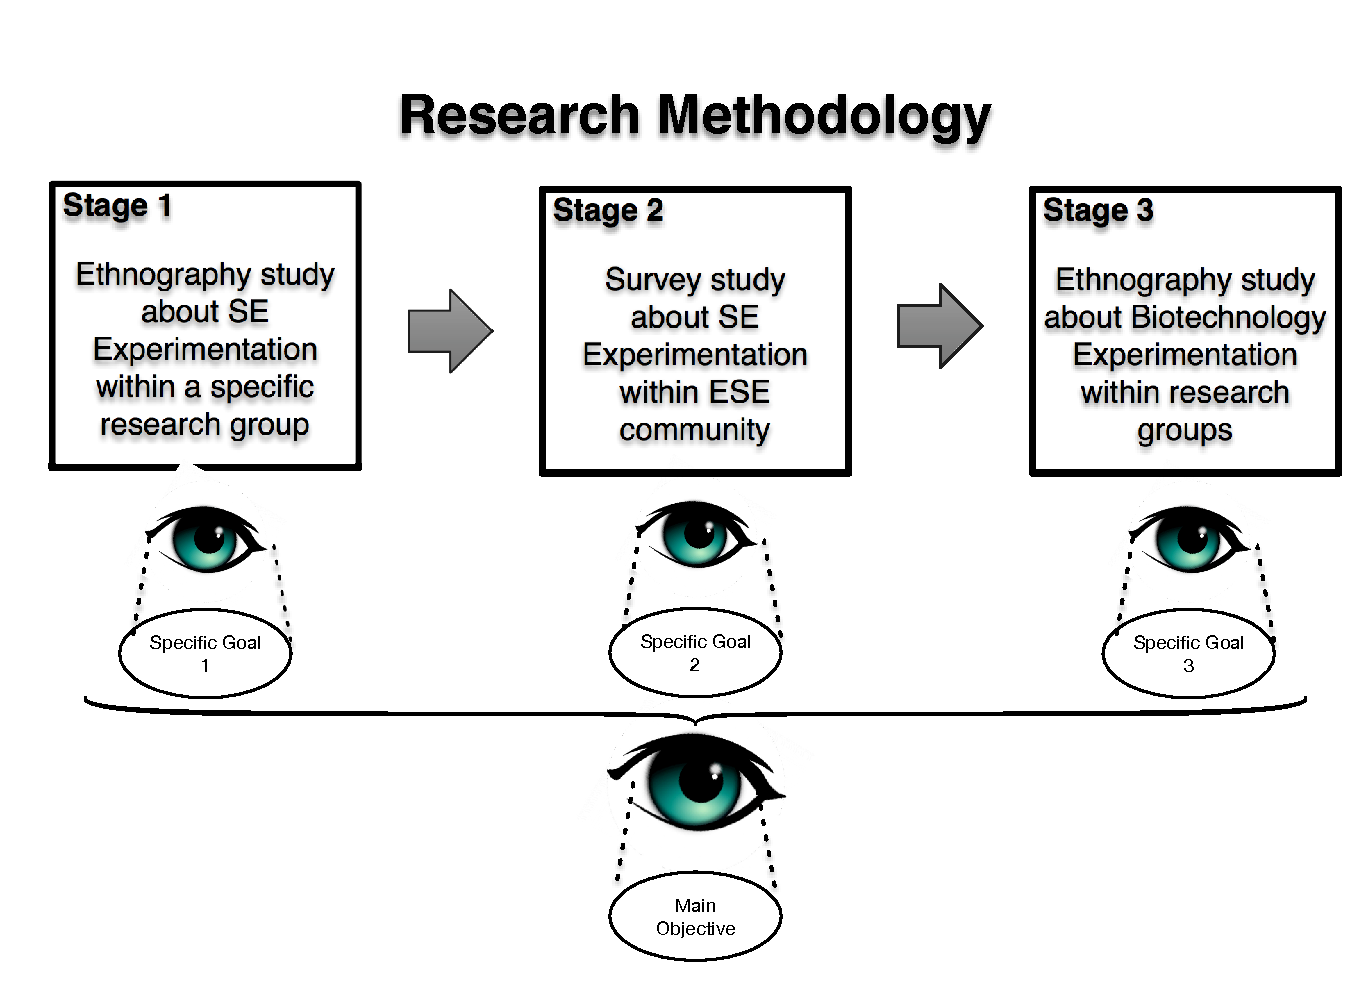
\includegraphics[width=10cm]{Images/Methodology}
	\caption{Research Methodology}
	\label{fig-research-methodology}
\end{figure*}

Los estudios etnogr�ficos pretenden dar respuesta a dos preguntas de investigaci�n concretas:

\begin{framed}%
\textbf{RQ1: How researchers conduct the SE experiments in practice into a specific research group?}
\end{framed}

\begin{framed}%
\textbf{RQ2: Is there deviation of the SE experimentation practice from traditional disciplines?}
\end{framed}

Para responder rigurosamente a estas preguntas, ser�a preciso realizar la investigaci�n en varias muestras del universo de grupos de investigaci�n de ambas disciplinas. Dado el alto costo que esto representa, la �nica alternativa factible ser�a la realizaci�n de un survey. Sin embargo, un survey podr�a sesgar la respuesta a las preguntas de investigaci�n, i.e., los experimentadores podr�an reportar lo que creen que hacen, en lugar de lo que realmente hacen. Este efecto ya ha sido observado anteriormente [REF].
 
Visto desde esta perspectiva, se precis� aplicar una aproximaci�n emp�rica de observaci�n para garantizar la fiabilidad de los resultados obtenidos, su validez y significancia cient�fica \cite{sjoberg-2007-future-empical-methods}. Por lo tanto, los m�todos factibles a ser utilizados eran: etnograf�a, action research o case study. Como esta investigaci�n precisaba estudiar c�mo se desarrolla la experimentaci�n en su entorno natural (grupos de investigaci�n), realizamos los ethnographical studies \cite{Sharp-2016-Ethnographic-Studies-ESE}.

Esta metodolog�a obliga a que la investigaci�n sea llevada a cabo en un peque�o n�mero de grupos de investigaci�n, lo que implica ciertos riesgos, dado que la validez de los resultados se ve amenazada. Para disminuir estos riesgos llevamos a cabo un riguroso proceso investigativo en contextos de experimentaci�n (i.e., grupos de investigaci�n) representativos de la poblaci�n bajo estudio (i.e., experimentadores en ESE y otra disciplina experimental asentada). Para aumentar la validez de nuestro estudio, triangulamos los resultados de la investigaci�n etnogr�fica con el survey antes citado, lo que nos permiti� responder a la siguiente pregunta de investigaci�n:

%\begin{framed}%
%\textbf{RQ3: To determine the generalizability of the experimentation process performed into a specific SE research group}
%\end{framed}

\begin{framed}%
\textbf{RQ3: �Cu�n generalizables son nuestros hallazgos a la comunidad de experimentadores en SE?}
\end{framed}

\subsection{Ethnographical Studies}
Los estudios etnogr�ficos se estructuraron en base a las gu�as de Per Runenson \cite{Runenson-2012-case-study-in-SE} para estudios de caso. Estas gu�as dan un soporte bastante espec�fico para las investigaciones que pretenden entender fen�menos que suceden en el mundo real; no obstante, es preciso tener presente que hacer una investigaci�n exhaustiva de este tipo en SE, no es una tarea f�cil.

El dise�o de los estudios etnogr�ficos consisten de: (1) Context selection, (2) Data collection procedures, y (3) Data analysis procedure.

\subsubsection{Context selection}
El criterio de selecci�n del contexto aplicado en los estudios etnogr�ficos parte de la premisa que un grupo de investigaci�n representativo constituye una fuente fiable de informaci�n, lo que facilita la tarea de aprendizaje respecto a la experimentaci�n. Por lo tanto, planteamos las siguientes condiciones como criterios de selecci�n del contexto:

\begin{itemize}
\item{Ser un grupo de investigaci�n cuyos experimentadores tengan una consolidada experiencia en el �rea}

\item{Ser un grupo de investigaci�n cuyos experimentadores sean reconocidos en la comunidad cient�fica a trav�s de publicaciones de alto impacto, tales como libros, art�culos, manuales t�cnicos, entre otras.)}
\end{itemize}

Dadas estas condiciones, los grupos seleccionados son, por una parte, el Grupo de Investigaci�n en Ingenier�a de Software Emp�rica (GrISE) perteneciente a la Escuela T�cnica Superior de Ingenieros Inform�ticos (ETSII) de la Universidad Polit�cnica de Madrid (PM) de Espa�a y por otra parte, tres grupos de investigaci�n de la Carrera de Biotecnolog�a de la Universidad de las Fuerzas Armadas ESPE de Ecuador. Una descripci�n detallada de los grupos de investigaci�n seleccionados se realiza en las Secciones \ref{sec-ESE-etnography} y \ref{sec-bio-etnography}, respectivamente.

\subsubsection{Data collection procedures}\label{subsec-data-collection}
El proceso de recolecci�n de informaci�n aplicado fue c�clico, iterativo e incremental, cuyas acciones fueron realizadas sobre distintas fuentes de informaci�n, con el prop�sito de indagar sobre la experimentaci�n llevada a cabo en los grupos de investigaci�n seleccionados.

Las fuentes generadoras de informaci�n corresponden espec�ficamente a aquellas accesibles y representativas dentro de los grupos de investigaci�n bajo estudio. Para la presente investigaci�n se consider� (en los casos que fue posible) a la: Literatura com�n del grupo (general y espec�fica), material experimental del grupo (general y espec�fico) y conocimiento de los experimentadores del grupo (internos y externos).

El orden en el que el investigador toma contacto con las fuentes de informaci�n es aleatorio. La frecuencia de contacto con las fuentes depende de la necesidad del investigador por cumplimentar el conocimiento; pero sobre todo, depende de la disponibilidad de cada fuente. Es decir, mientras m�s disponible es la fuente, el investigador se mantiene m�s tiempo en contacto con la misma. A continuaci�n se detalla la interacci�n del investigador con cada fuente.

\begin{itemize}
  \item En lo que respecta a la literatura com�n del grupo, el investigador tiene acceso a la misma de forma inmediata y continua en el tiempo, a trav�s de bibliotecas, bases digitales disponibles, versiones impresas disponibles, entre otras. La literatura representa una fuente de informaci�n muy importante, dado que proporciona la informaci�n referente al proceso de experimentaci�n, desde la perspectiva te�rica.
 
  \item El contacto con el material experimental m�s representativo y fiable propio del grupo de investigaci�n es inmediato y continuo en el tiempo, con la gu�a de los experimentadores. Sin embargo, para facilitar el proceso de revisi�n y aprendizaje de la informaci�n contenida en esta fuente, se precisa un contacto previo con la literatura com�n del grupo. Eventualmente es preciso el estudio de material espec�fico para profundizar en una tem�tica particular. El material experimental representa la evidencia de la experimentaci�n llevada a cabo en la pr�ctica por el grupo de investigaci�n.

  \item La obtenci�n del conocimiento de los experimentadores es planificada en funci�n de su disponibilidad de tiempo. Este proceso se realiza desde un inicio, ya que se representa una alta complejidad, considerando la aplicaci�n de distintas t�cnicas e instrumentos. Para el caso de los experimentadores externos, no es posible una planificaci�n espec�fica, dada la dificultad de un contacto directo; por lo tanto, en este punto mucho se depende de la casualidad. El conocimiento obtenido de los experimentadores, representa el proceso de experimentaci�n realizado en la practica dentro de los grupos de investigaci�n. 
\end{itemize}

El conocimiento obtenido de las fuentes indicadas se complement� entre si y sirvi� para determinar en qu� medida lo que se encuentra expresado en la teor�a, corresponde a lo que efectivamente llevan a cabo los experimentadores en la pr�ctica dentro de los grupos de investigaci�n.

Para el proceso de extracci�n de la informaci�n se utiliz� una taxonom�a de t�cnicas de recolecci�n de informaci�n, categorizada de acuerdo al nivel de contacto con la fuente primaria de informaci�n. La taxonom�a propone tres niveles de recolecci�n de informaci�n: Participaci�n directa con la fuente (nivel 1), participaci�n indirecta con la fuente (nivel 2) y estudio del material de trabajo (sin la participaci�n de la fuente) (nivel 3) \cite{Lethbridge-2005-studyingsoftwaredatacollection}.

El procedimiento para la recolecci�n de informaci�n de las fuentes indicadas, consiste en aplicar t�cnicas adecuadas dependiendo del tipo de fuente y de su disponibilidad. Por ejemplo, para extraer informaci�n de los experimentadores de un entorno de experimentaci�n se utilizaron t�cnicas tales como: entrevistas, grupos de discusi�n, entre otros (primer nivel). La adecuada aplicaci�n de las t�cnicas de recolecci�n de informaci�n se asocia a la utilizaci�n de diferentes instrumentos, algunos de los cuales se constituir�n como piezas fundamentales para recrear la informaci�n obtenida. Por ejemplo utilizamos: videoc�maras, dispositivos de grabaci�n de audio, entre otros. M�s espec�ficamente, las t�cnicas de recolecci�n de informaci�n aplicadas a las fuentes de informaci�n, se indican en la Tabla \ref{tbl-tecnica-fuente}.

\begin{table}
	\centering
	\caption{T�cnicas de recolecci�n por fuente de informaci�n}
	\label{tbl-tecnica-fuente}
	\begin{tabular}{|p{3.7cm}|p{3.7cm}|}
	\hline
	\textbf{Fuente} & \textbf{T�cnicas}\\
	\hline
	\multirow{7}{50 pt}{Conocimiento del grupo de investigaci�n} & Entrevistas\\
	\cline{2-2}
	& Grupos de discusi�n\\
	\cline{2-2}
	& Observaci�n participativa\\
	\cline{2-2}
	& Modelado de actividades\\
	\cline{2-2}
	& Sistemas instrumentales\\
	\cline{2-2}
	& Aprendizaje basado la experiencia\\
	\hline
	\multirow{1}{85 pt}{Literatura referente} & An�lisis de documentaci�n\\
	\hline
	\multirow{1}{95 pt}{Material experimental} & An�lisis de documentaci�n\\
	\hline
	\multirow{3}{95 pt}{Conocimiento de experimentadores} & Entrevistas\\
	\cline{2-2}
	& Grupos de discusi�n\\
	\cline{2-2}
	& Sistemas instrumentales\\
	\hline
	\end{tabular}
\end{table}
 
Los inconvenientes presentados por el uso de las diferentes t�cnicas e instrumentos fueron minimizados gracias a su combinaci�n en cada iteraci�n. Por ejemplo, los vac�os del audio fueron complementados por el video, las fotograf�as y los esbozos de los experimentadores y viceversa.

\subsubsection{Data analysis procedure}
El procedimiento de an�lisis de datos tiene un enfoque cualitativo y est� asociado con la aplicaci�n de las t�cnicas de obtenci�n de informaci�n, por lo que fue iterativo incremental. El n�mero de iteraciones de an�lisis corresponde al n�mero de iteraciones de recolecci�n de datos realizado con cada fuente. El procedimiento de an�lisis (ver Figura \ref{fig-proc-analisis}) se compone de dos actividades principales: (1) Verificaci�n de los datos y (2) Comparaci�n de los datos.

\begin{figure}[htbp!]
	\centering
	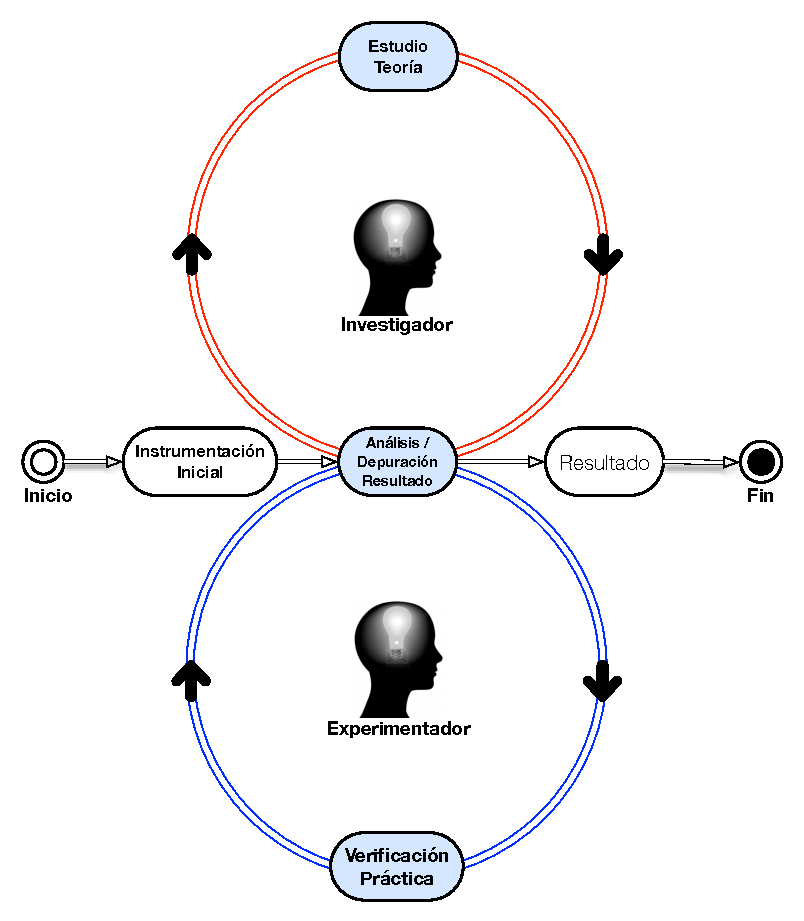
\includegraphics[width=2.5in]{Images/proceso-analisis}
	\caption{Proceso de An�lisis}
	\label{fig-proc-analisis}
\end{figure}

La actividad de verificaci�n de datos tiene como prop�sito verificar la validez de la informaci�n recolectada como insumo para el an�lisis, lo cual ser� realizado principalmente por los mismos experimentadores del grupo bajo estudio. Durante las revisiones de las fuentes te�ricas, los investigadores fueron adquiriendo paulatinamente conocimientos b�sicos de la experimentaci�n, lo cual les sirvi� para entender m�s f�cilmente los resultados obtenidos de la interacci�n con el conocimiento de los experimentadores. Los resultados obtenidos fueron expresados de forma expl�cita en medios f�sicos o digitales y validados por los experimentadores en cada iteraci�n hasta obtener el resultado final.
 
Comparaci�n de los datos: La comparaci�n de los datos obtenidos fue realizada tanto por los investigadores como por los experimentadores en una actividad de revisi�n cruzada, cada vez que se realiz� la verificaci�n de los datos en los resultados intermedios obtenidos. Por un lado los investigadores hacieron la comparaci�n del resultado con su conocimiento adquirido de la revisi�n de otras fuentes de informaci�n; mientras que los experimentadores compararon el resultado con las actividades que efectivamente realiza en la pr�ctica.

\subsection{Survey of the experimentation process in SE}
Para validar los hallazgos del estudio sobre el proceso de experimentaci�n en SE dentro de un grupo de investigaci�n, realizamos un survey en la comunidad de ESE. Siguiendo los 

\subsubsection{Introduction}
This research is intended to study the underlying problems surrounding the ESE and inquire about their possible origins. To do this, we carried out an empirical study based on a structured survey, in order to obtain insight of the most representative researchers into the Empirical Software Engineering Community. From this point of view, we have considered survey the researchers whose articles have been accepted in the most representative symposiums, workshops or conferences, such as: the ``Symposium on Empirical Software Engineering and Measurement" (ESEM), the Experimental Software Engineering Latin America Workshop (ESELAW), among others.

\subsubsection{Survey's Goal}
This research aims to study the underlying problems surrounding the Experimentation in Software Engineering and find out their possible origins. This study will be carried out through a structured survey in the context of the ESEM and ESELAW symposiums.

With the purpose of contextualize the survey's goal, the following research questions were proposed.

\begin{framed}%
\textbf{RQ1: What are the circumstances in which SE researchers obtained their base training on experimentation and what is their current experience?}
\end{framed}

\begin{framed}%
\textbf{RQ2: How is the experimental process in Software Engineering?}
\end{framed}

\begin{framed}%
\textbf{RQ3: What problems are faced by researchers during experimental software engineering process?}
\end{framed}

\begin{framed}%
\textbf{RQ4: What instances of experimental process need improvement from the point of view of Software Engineering researchers?}
\end{framed}

\subsubsection{Target Population}
Software Engineering researchers whose papers were accepted in ESEM 2016 symposium, and researchers who usually published in the CIbSE conference's track named ESELAW.

\subsubsection{Sampling Design}
The website (based on a survey) used to operationalize the study will be published through flyers and email to our target population. Advertising aims to capture the attention of researchers to implement the survey.

\subsubsection{Survey's Questions}



\section{Experimentation In Software Engineering}\label{sec-ESE-etnography}

\odnote{Tendremos que discutir con Natalia si debemos hacer an�nimos los grupos. Teniendo en cuenta lo que se dice, creo que es justificable. Una aproximaci�n posible es hacer que los grupos sean conocidos para los revisores, pero no para los lectores.}

El estudio fue realizado en el Grupo de Investigaci�n en Ingenier�a de Software Experimental (GrISE) de la Universidad Polit�cnica de Madrid (UPM). GrISE es un grupo que puede considerarse representativo de la comunidad de ESE. El origen del grupo data de finales de los 90s, cuando fue fundado por N. Juristo, una investigadora reconocida en IS por su temprano libro (con A. Moreno) acerca de SE experimental \cite{Juristo2001} , adem�s de sus contribuciones posteriores. El grupo cuenta con otros investigadores de dilatada trayectoria, tales como O. Dieste y S. Vegas. A lo largo de su historia, GrISE ha realizado varias familias de experimentos \cite{Basili1999-KnowledgeFamiliesExp}, en distintas tem�ticas: testing (�ntimamente relacionada con los experimentos iniciados por Basili y colaboradores, tales como \odnote{RODRIGO: A�adir}), requisitos (\odnote{RODRIGO: A�adir; pregunta a Oscar}) y, m�s recientemente, test-driven development (e.g., \odnote{RODRIGO: A�adir}).

El estudio se desarroll� por fases iteradas, tal y como se puede observar en la Figura \ref{fig-process-etnography-study1}. Las fases no se planificaron de antemano, sino que  que se plantearon sobre la base de los hallazgos obtenidos durante la investigaci�n, tal y como describiremos a lo largo de esta secci�n. La descripci�n tendr� un car�cter denso\footnote{A 'dense' or 'thick' description is a reporting style in Ethnography in which the research findings are explicitly related to their occurring context. A dense description faciliates the critical evaluation of the findings, e.g., their external validity, by enabling the comparison to other contexts. For instance, see \cite{}\odnote{Usar la referencia \url{https://books.google.es/books?id=8BU63Xf2JGQC}, pp. 60-62}.}, tal y como es habitual en Etnograf�a. El lector encontrar� fragmentos subrayados; dichos fragmentos representan, en nuestra opini�n, hallazgos importantes de la investigaci�n etnogr�fica. Dichos hallazgos se recopilan y discuten en la Secci�n~\ref{sec-discussion-conclusions}.

\begin{figure}[htbp!]
	\centering
	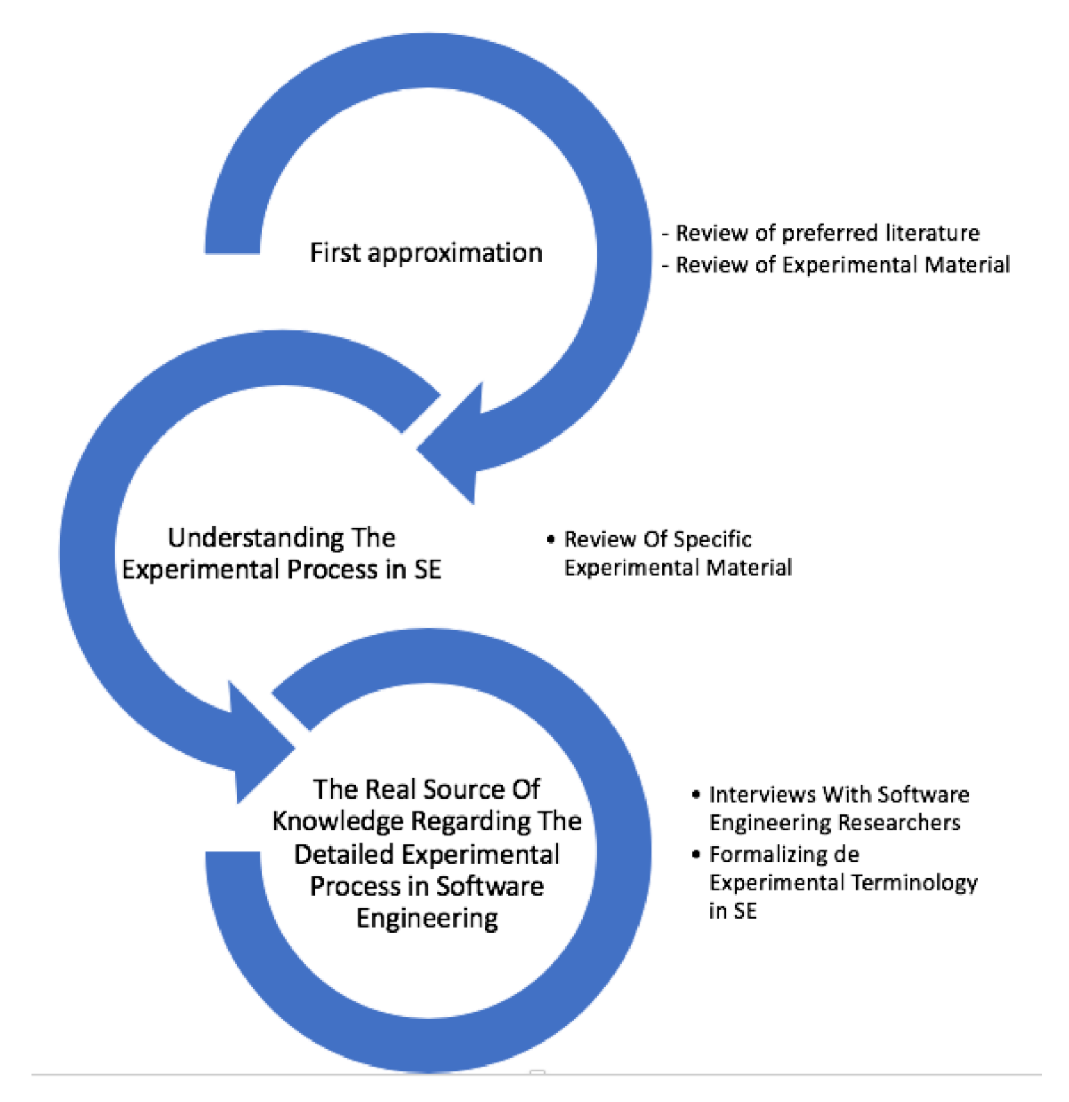
\includegraphics[width=3.2in]{images/Etnogaphy1-Process}
	\caption{Fases del Estudio Etnogr�fico de la Experimentaci�n en SE}
	\label{fig-process-etnography-study1}\odnote{RODRIGO: El t�tulo del tercer c�rculo me parece muy complejo. La lista de vi�etas deber�a estar en un texto un poco m�s grande, para que se lea mejor.}
\end{figure}

\subsection{First Approximation}\label{subsec-results-case1}

 \odnote{RODRIGO: Hay que clarificar quienes somos "nosotros". En alg�n lugar debemos dejar dicho el modo en que vamos a denominar a los investigadores de los grupos y a los autores de esta investigaci�n.}

La primera actividad que realizamos fue entrevistar a los miembros del GrISE. El objetivo de las entrevistas era adquirir el conocimiento del grupo y volcarlo en modelos conceptuales que permitiese su an�lisis y manipulaci�n posterior. \odnote{RODRIGO: Proporcionemos cierto contexto:} {\color{green}Realizamos XXX entrevistas (no deber�an ser muchas....). A estas entrevistas acudieron....}

Pronto se evidenci� que las entrevistas iban a ser insuficientes para alcanzar este objetivo. Los miembros del GrISE nos proporcionaron cierto conocimiento expl�cito, en particular los componentes principales de un experimento (hip�tesis, factor, nivel, etc.). Sin embargo, no result� posible profundizar demasiado m�s:

\odnote{OSCAR: Los {\color{blue}(?)} hay que procesarlos al final de la revisi�n. Quiz�s no sean hallazgos fidedignos.}

\begin{itemize}

\item Los miembros del GrISE cre�an que las entrevistas eran innecesarias, ya que el conocimiento que busc�bamos pod�amos adquirirlo por nosotros mismos en {\color{blue}(?)} \ul{literatura que ellos consideraban est�ndar}, e.g., \cite{Wohlin2000}.

\item A medida que profundiz�bamos en algunas �reas, e.g., planificaci�n experimental o gesti�n de datos, los miembros del GrISE necesitaban {\color{blue}(?)} \ul{apoyar su relato con ejemplos concretos}, que obten�an de su propio material experimental, lo que dificultaba la comunicaci�n ya que nosotros desconoc�amos dichos materiales.

\end{itemize}

El estudio de ambas fuentes result� imprescindible para proseguir la interacci�n con los miembros del GrISE.

\subsubsection{An�lisis de la literatura relevante}\label{subsubsec-study-literature}

Los miembros del GrISE se�alaron como {\color{blue}(39)} \ul{fuentes b�sicas de su proceso experimental los libros} by Wohlin et al. \cite{Wohlin2000} and Juristo \& Moreno. \cite{Juristo2001}. El GrISE tambi�n {\color{blue}(40)} \ul{utiliza como fuentes b�sicas ciertos reportes o art�culos espec�ficos}. Resultan especialmente relevantes los textos de Basili et al. \cite{Basili-1986-ESE} y Kitchenham et al. \cite{Kitchenham2002-GuideLinesESE}, los cuales representan recomendaciones tempranas acerca de c�mo experimentar en SE. En el caso particular del GrISE, dado su inter�s por realizar replicaciones experimentales, resulta tambi�n especialmente relevante el trabajo de Basili et al. \cite{Basili1999-KnowledgeFamiliesExp}.

La literatura fue revisada en profundidad por los dos investigadores principales (E. Fonseca y E. Espinosa). El primer aspecto que nos llam� la atenci�n fue la {\color{blue}(2)} \ul{diversidad terminol�gica con que las distintas fuentes se refer�an a actividades similares del proceso experimental}. Para nosotros, observadores sin conocimientos espec�ficos de experimentaci�n, la literatura parecer�a describir distintos tipos de experimentos, cada uno caracterizado por un proceso diferente. A modo de ejemplo, los materiales antes citados \cite{Wohlin2000,Juristo2001,Basili-1986-ESE,Kitchenham2002-GuideLinesESE} denominan las fases del proceso de experimentaci�n en SE de formas diversas:

\begin{itemize}
	\item Wohlin et al. \cite{Wohlin2000} \textquotedblleft proponen como fases del proceso experimental: Experiment idea, Experiment scoping, Experiment planning, Experiment operation, Analysis \& interpretation, Presentation \& package and Experiment report\textquotedblright.
	\item Juristo \& Moreno \cite{Juristo2001}: \textquotedblleft Objective Definition, Design, Execution and Analysis\textquotedblright.
	\item Basili et al. \cite{Basili-1986-ESE}: \textquotedblleft Definition, Planning, Operation, and Interpretation\textquotedblright.
	\item Kitchenham et al. \cite{Kitchenham2002-GuideLinesESE}: \odnote {RODRIGO: A�adir}
\end{itemize}

Aunque los autores definen estas fases en detalle, la coincidencia en t�rminos y descripci�n difiere mucho de uno a otro autor. Una vez adquiridos conocimientos acerca experimentaci�n en SE es inmediato percibir las similitudes, pero a�n as� {\color{blue}(?)} \ul{no est� claro si los distintos autores est�n describiendo exactamente las mismas actividades}.

Hemos buscado libros de texto complementarios a \cite{Wohlin2000,Juristo2001}, con la intenci�n de verificar si la diversidad terminol�gica era un problema general, o estaba circunscrito a las fuentes recomendadas. S�lo hemos localizado la nueva edici�n del libro de Wohlin et al. \cite{Wohlin2012-Experimentation} sobre experimentaci�n, y los libros especializados de Runeson et al. \cite{case-study-in-SE-Runenson-2012} y Kitchenham et al. \cite{Kitchenham-2015-Literature-Review-Book}. Preguntados a este respecto, los miembros del GrISE nos se�alaron otras fuentes, tales como Box et al. \cite{Box2008}, Montgomery \& Runger \cite{montgomery-2010-applied-statistics} o \odnote{a�adir \url{https://books.google.es/books?id=srb0a9fmMEoC}}, pero en seguida nos aclararon que se trataban de libros dirigidos m�s al an�lisis estad�stico que a la planificaci�n y dise�o experimentales. En consecuencia, creemos poder afirmar que la {\color{blue}(5)} \ul{carencia de textos de referencia} es un aspecto caracter�stico de la experimentaci�n en SE.

Nuestro objetivo inicial, como ya hemos indicado anteriormente, era adquirir el conocimiento del grupo y volcarlo en modelos conceptuales. Aunque la literatura no era coherente entre s�, conseguimos crear, con la ayuda de los miembros del GrISE, el modelo conceptual preliminar que se muestra en la Fig.~\ref{fig-conceptos-preliminar}. Este modelo contiene conceptos que ahora reconocemos de muy alto nivel de abstracci�n, tales como: Experimento, Replicaci�n, S�ntesis, Hip�tesis, Variables, Dise�o Experimental, etc., pero suficientes en aquel entonces para continuar con la investigaci�n etnogr�fica.

\begin{figure*}[htbp!]
	\centering
	\captionsetup{justification=centering}
	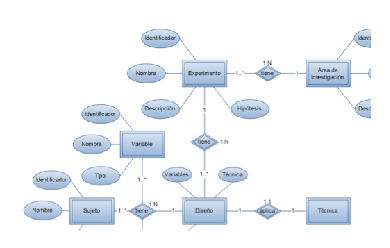
\includegraphics[width=5in]{images/Producto-Intermedio-Revision-Lit}
	\caption{Modelo conceptual preliminar resultado de la primera aproximaci�n.}
	\label{fig-conceptos-preliminar}
	\odnote{RODRIGO: Agranda la figura. Que se vea todo si es posible. Quiero que se vea como las ideas van cambiando a lo largo de la investigaci�n.}
	\odnote{RODRIGO: Si las figuras van en el texto, habr� que traducirlas al ingl�s. Si van en anexo, yo no las traducir�a, porque los materiales de la investigaci�n (incluyendo el material que tienes online) est� en Espa�ol.}
\end{figure*}

\subsubsection{Review of experimental material}\label{subsubsec-study-material}

El estudio del material experimental de GrISE constituy� una fuente de informaci�n valiosa, ya que refleja el conocimiento t�cito presente en el grupo, gestado durante m�s de una d�cada de experimentaci�n. El material es variado; se compone fundamentalmente de: planteamientos de experimentos, dise�os, instrumentos experimentales (e.g.: formularios de tareas experimentales, formularios de recogida de datos, gu�as), objetos experimentales (e.g.: programas con faltas sembradas, especificaciones de requisitos alteradas con anomal�as), raw data (e.g.: hojas de excel con datos de mediciones de tareas experimentales realizadas, bases de datos), material de entrenamiento (e.g.: manuales t�cnicos, presentaciones) y, finalmente, publicaciones (e.g.: \cite{Juristo2012-EffectivenessWithinOutsideScopeExperiment,Juristo2006-SoftwareTestingTechniques,Juristo-2003-ESERNET}).

El primer problema que nos encontramos fue el acceso al material experimental, dado que {\color{blue}(12)} \ul{no existe una pol�tica de gesti�n del material}. Un ejemplo paradigm�tico son los raw data. Encontramos raw data en distintos tipos de ficheros, correspondientes a distintas versiones, {\color{blue}(9)} \ul{cuya ubicaci�n y formato son conocidos �nicamente por la persona que los gestiona}. Lo mismo puede afirmarse de los restantes tipos de materiales, incluidas las publicaciones; de no existir librer�as digitales, algunas incluso podr�an no haber estado accesibles.

Fue preciso solicitar ayuda a los miembros del GrISE para acceder al material experimental, entender su estructura y evoluci�n temporal. Revisamos primero lo m�s antiguo, avanzando progresivamente hacia la actualidad. La revisi�n fue apoyada el albacea de la informaci�n, cuyo relato sumado a la informaci�n obtenida del material revisado, nos permiti� descubrir que  {\color{blue}(10)} \ul{las actividades que generaron el material experimental han ido evolucionando y mejorando con el tiempo}. Ello se debe fundamentalmente a: (1) la mayor experiencia y conocimientos acerca de experimentaci�n que el grupo ha obtenido con el paso del tiempo y (2) la mayor exigencia de los revisores, los cuales han mejorado igualmente su pericia progresivamente.

Otro aspecto que nos llam� la atenci�n en la revisi�n del material experimental, fue la complejidad del planteamiento de los experimentos. Los documentos del GrISE se caracterizan por {\color{blue}(14)} \ul{realizar una descripci�n general de las actividades a ser realizadas en el experimento, pero no proporcionan una gu�a clara sobre el orden de ejecuci�n y relaci�n entre actividades experimentales}. Por ejemplo, encontramos planteamientos de experimentos que inclu�an un dise�o experimental, mientras que otros no. Cuando el dise�o experimental estaba presente, no se acostumbraba a indicar su tipo, sino �nicamente su estructura y conformaci�n (e.g., las tabla presente en \cite[pp. 92]{Juristo2001}).

Ya hemos mencionado que GrISE ha realizado distintas familias de experimentos. La comparaci�n de los materiales relativos a distintas familias (e.g., testing vs. requirements) pose�an marcadas diferencias. Estas diferencias eran de dos tipos:

\begin{itemize}

\item El procedimiento experimental depend�a en gran medida de la familia. \odnote{RODRIGO: Podr�amos poner ejemplos de diferencias, quiz�s entre las familias de testing y requisitos? Mira la secci�n \ref{conduccion-replicacion} para que no repitamos el mismo argumento}. Parece que {\color{blue}(13)} \ul{existe una diversidad de aproximaciones y enfoques sobre la realizaci�n de experimentos}, dependiendo de la familia y el investigador que los plantee.

\item Los materiales hac�an referencia a t�rminos totalmente diferentes a los identificados hasta el momento en la literatura, tales como: \textit{efecto del cansancio}, \textit{efecto del aprendizaje}, etc. Poniendo en contraste la literatura y el material experimental revisados, estaba claro que {\color{blue}(34)} \ul{los reportes sufr�an incluso mayor diversidad terminol�gica que los libros de referencia}. Dependiendo de la familia, encontramos definiciones similares usando t�rminos diferentes, los mismos t�rminos con definiciones diferentes, y t�rminos diferentes con definiciones diferentes referidas al mismo concepto.

\end{itemize}

Con el prop�sito de mejorar el modelo conceptual mostrado en la Fig.~\ref{fig-conceptos-preliminar}: (1) conservamos los conceptos que se manejan en GrISE y, (2) para el caso de los conceptos nuevos, optamos por utilizar los t�rminos m�s comunes entre las fuentes revisadas, independientemente de la opini�n de los miembros del grupo. El resultado fue el modelo conceptual que se muestra en la Fig.~\ref{fig-conceptos-final-revision-fuentes}. \odnote{RODRIGO: Habr�a que comentar las diferencias principales entre la Fig.~\ref{fig-conceptos-preliminar} y la Fig.~\ref{fig-conceptos-final-revision-fuentes}.}

\begin{figure*}[htbp!]
	\centering
	
\includegraphics[width=5in]{images/Producto-Final-Revision-Lit}
	\caption{Modelo conceptual resultado del an�lisis de los materiales experimentales.}
	\label{fig-conceptos-final-revision-fuentes}\odnote{RODRIGO: Pon el modelo completo. Quiz�s haya que mover estos gr�ficos a un anexo.}
\end{figure*}

\subsection{Understanding the experimental process in SE}\label{subsec-second-aprox}

Un aspecto diferencial de la etnograf�a frente a otras metodolog�as de investigaci�n cualitativas es la \textit{observaci�n participativa}. Los investigadores etnogr�ficos deben adoptar "el punto de vista de los nativos" para entender mejor el motivo de sus acciones \cite{}\odnote{Usar la referencia \url{https://books.google.es/books?id=8BU63Xf2JGQC}, pp. 55-56}. En nuestro caso, la incertidumbre surg�a de la diversidad terminol�gica y operativa observada en los materiales experimentales. En consecuencia, nos planteamos realizar nosotros mismos un experimento.

\subsubsection{Selecci�n del experimento}\label{seleccion-del-experimento}

En lugar de dise�ar un experimento desde el principio, nos pareci� preferible replicar un experimento previamente realizado por el grupo. Hab�a dos motivos para ello:

\begin{itemize}

\item Realizar una replicaci�n despertaba el inter�s de los miembros del GrISE, lo que nos aseguraba su colaboraci�n.

\item La replicaci�n nos permitir�a recrear el dise�o, ejecuci�n, an�lisis y reporte de un experimento que hasta entonces s�lo hab�amos conocido mediante el examen de material escrito, lo que a su vez nos permitir�a entender mejor las motivaciones y decisiones tomadas en aquel entonces por los experimentadores.

\end{itemize}

The selected baseline experiment \cite{Juristo2012-EffectivenessWithinOutsideScopeExperiment} belongs to the testing family. La replicaci�n se llev� a cabo en la Universidad de la Fuerzas Armadas ESPE, Sede Latacunga (Ecuador), y fue publicada posteriormente \cite{Fonseca-2013-Replication-Efectiveness-In-Out}.

\subsubsection{Planificaci�n de la replicaci�n}\label{planificacion-replicacion}

Se ha indicado repetidas veces en la literatura la dificultad de realizar replicaciones experimentales \cite{}\odnote{RODRIGO: Hay que indicar referencias}. Los motivos aducidos son variados: \odnote{RODRIGO: Indicar}. En nuestro caso, el principal problema fue {\color{blue}(14)} \ul{la carencia de una gu�a detallada de las actividades experimentales a realizar}, hecho que ya hab�amos observado anteriormente (en la Secci�n~\ref{subsubsec-study-material}).

Para planificar la replicaci�n, fue necesario contar con la participaci�n directa de los investigadores que realizaron el experimento original (N. Juristo y S. Vegas).

\odnote{RODRIGO: Esta descripci�n me parece muy simple. Podr�as darle un poco m�s de riqueza? Qu� os dijeron? Qu� no entend�steis? Quiz�s creaste alg�n modelo de resumen de lo que os contaron?}

\begin{tcolorbox}

Su aporte principal fue \textit{guiar el dise�o experimental, el uso del material experimental y dar los lineamientos espec�ficos para realizar la ejecuci�n y an�lisis del experimento}{\color{blue}(28)}. 

\end{tcolorbox}

\subsubsection{Conducci�n de la replicaci�n}\label{conduccion-replicacion}

\odnote{RODRIGO: Es esto verdad?}

La replicaci�n fue realizada por R. Fonseca. No hubo incidentes dignos de consideraci�n. La gu�a proporcionada por N. Juristo y S. Vegas fue suficiente para comprender y ejecutar con �xito, o al menos as� lo creemos, las distintas actividades del experimento. La existencia de materiales experimentales precisos (cuestionarios, descripciones de las tareas, programas, etc.) facilit� sobremanera la realizaci�n del experimento, ya que todas los aspectos relevantes estaban definidos de antemano.

Los materiales experimentales no son siempre tan precisos como en el caso de la familia de testing. Como ya hemos reportado en la Secci�n~\ref{conduccion-replicacion}, los documentos de la familia de requisitos eran mucho menos detallados que los de la familia de testing. Seg�n nuestra experiencia con la replicaci�n de experimento de testing, dicha falta de detalle s�lo pod�a perjudicar la conducci�n del experimento. 

El experimentador responsable de la familia de requisitos, O. Dieste, nos explic� que el {\color{blue}(?)} \ul{tipo y nivel de detalle de los materiales experimentales estaba en relaci�n a las tareas que los sujetos deb�an realizar}. Por ejemplo, las preguntas que pueden surgir en un experimento en elicitaci�n mediante entrevistas son muy diversas, y no se puede preparar de antemano una respuesta para cada una de ellas. En contrapartida, en la familia de testing todos los sujetos realizaban m�s o menos la misma tarea de la misma forma, e.g., dise�o de casos de prueba mediante partici�n de equivalencia, lo que permit�a proporcionar a los sujetos, e.g., instrucciones m�s precisas.

\subsubsection{Medici�n}\label{medicion-replicacion}

Por el contrario, la medici�n de los resultados result� m�s complicada. La raw data del experimento se obten�a a partir de test cases propuestos por los sujetos experimentales, los cuales pod�an detectar o no una determinada falta. El problema fundamental era que los test cases no se ejecutaban, sino que se evaluaban por los medidores (en este caso, R. Fonseca y E. Espinosa). Para completar la medici�n fue necesario consultar con los miembros del GrISE, y a�n as� {\color{blue}(?)} \ul{se produjo un cierto grado de ambig�edad en la generaci�n del raw-data}. \odnote{RODRIGO: Es esto cierto?} Por el contrario, los restantes pasos de la medici�n (c�lculo de medidas a partir de la raw-data, y formateo de los datos para an�lisis) no implicaron ninguna incertidumre. 

\subsubsection{An�lisis y reporte}\label{analisis-reporte-replicacion}


 O. Dieste, que no ha realizado experimentos en testing, proporcion� soporte en la conducci�n, an�lisis y reporte. 


No obstante, los resultados de la replicaci�n tuvieron diferencias marcadas con respecto al experimento original, incluso existieron errores en el an�lisis de resultados; posiblemente debido a factores propios del contexto donde se llev� a cabo la replicaci�n, o por falta de experiencia de quienes ejecutaron y analizaron los resultados de la replicaci�n. Esto indica que el conocimiento m�s granular sobre la ejecuci�n y an�lisis del experimento contenido en los lineamientos dados por los miembros del GrISE, al parecer no fue abstra�do del todo, confirm�ndose que \textit{no existe una gu�a clara y auto sustentable que permita realizar una replicaci�n literal, externa e independiente del experimento original, siendo necesaria la presencia de los experimentadores originales en todo el proceso de la replicaci�n}{\color{blue}(29)}.

\subsubsection{Evaluaci�n de la observacion participativa}\label{evaluacion-observacion-participativa}

Evaluando las actividades realizadas hasta el momento en la investigaci�n, encontramos que posiblemente el contenido de los textos de experimentaci�n revisados representen de forma expl�cita una parte del conocimiento de sus autores; sin embargo, comparando dicho contenido con los elementos del material experimental del GrISE, y con las actividades que no estaban indicadas en el material espec�fico revisado, y que nos fueron aclaradas para poder realizar la replicaci�n; vimos que las diferencias son muy marcadas, lo que muestra \textit{la generalidad de los textos, la falta de detalle del material experimental y la presencia de un conocimiento t�cito particular de cada investigador}{\color{blue}(8)}; esto se confirma por la necesidad permanente de contar con la gu�a de los miembros del GrISE. Sin duda alguna las aproximaciones realizadas nos permitieron adquirir un conocimiento importante de la experimentaci�n en SE, pero era claro que el conocimiento m�s granular del proceso experimental no lo hab�amos adquirido a�n. Nuestro nuevo camino a seguir estaba claro, intentar hacer expl�cito el conocimiento sobre experimentaci�n en SE de los miembros del GrISE.

\odnote{RODRIGO: Hay alg�n material que podamos poner como resultado de esta fase. Un mapa de procesos quiz�s? Un modelo conceptual refinado?}

\subsection{The Real Source Of Knowledge Regarding The Detailed Experimental Process in Software Engineering}\label{subsec-conocimiento-grupo}
Nuestro principal prop�sito ahora era hacer expl�cito el conocimiento granular de la experimentaci�n en SE que poseen los miembros del GrISE, lo cual no hab�a sido realizado anteriormente, seg�n nos indicaron. En primera instancia la tarea nos pareci� realizable, ya que pudimos concretar citas peri�dicas tanto para entrevistas personales, as� como para reuniones grupales de discusi�n. Sin embargo, en la pr�ctica tuvimos el mismo problema de acceso que con las otras fuentes de informaci�n revisadas, dado la inestable agenda que manejan los miembros del GrISE. Sin duda, esto complic� la fluidez de obtenci�n de informaci�n y sobre todo incidi� constantemente en la planificaci�n de las entrevistas y m�s a�n en las reuniones grupales de discusi�n. 

\subsubsection{Interviews With Software Engineering Researchers}\label{subsubsec-interviews-ESE}
Las entrevistas a los miembros del GrISE se sustentaron en un cuestionario simple de preguntas abiertas orientadas a conocer a detalle las actividades que lleva a cabo cada miembro dentro del proceso experimental. El cuestionario se enfoc� en motivar en el entrevistado un relato libre y abierto sobre su rol en el proceso. En las primeras sesiones se afin� la t�cnica de abstracci�n de conocimiento para obtener el mayor detalle posible. Por ejemplo, se pas� de utilizar pluma y papel para tomar nota de las respuestas de los entrevistados, a grabaciones de audio y video; de esta manera, el proceso implementado permiti� capturar los detalles m�s granulares del entrevistado referidos a lo expresado, a los gestos, e incluso a los rasgos con los que algunos entrevistados esbozaban su relato (por ejemplo ver Figura \ref{fig-proceso-exp-boseto}).

\begin{figure}[htbp!]
	\centering
	\includegraphics[width=3.2in]{images/Boseto-Proccess}
	\caption{Extracto de las actividades experimentales realizadas por los experimentadores del GrISE en boceto}
	\label{fig-proceso-exp-boseto}
\end{figure}

El conocimiento abstra�do en cada sesi�n de entrevistas fue validado con el mismo entrevistado al inicio de la sesi�n posterior. El conocimiento abstra�do fue presentado al entrevistado en formato impreso, cuyo contenido en su mayor�a era texto; a diferencia de la informaci�n obtenida de la entrevista a la fundadora del GrISE, quien adicion� en su relato un boceto sobre las actividades del proceso experimental, el cual fue recreado con herramientas inform�ticas (ver Figura \ref{fig-proceso-exp-boseto}). El detalle del proceso experimental obtenido de forma inesperada en esta entrevista en particular, nos dej� claro que \textit{los experimentadores de mayor experiencia tienen un conocimiento m�s amplio y detallado sobre las actividades que se llevan a cabo en la experimentaci�n en SE}{\color{blue}(21)}.

Las iteraciones de cada entrevista permitieron depurar los resultados, tanto en relato escrito como gr�fico (por ejemplo ver Figura \ref{fig-proceso-draft}) y terminaron tanto en cuanto los entrevistados indicaron que su relato sobre las actividades hab�a sido del todo hecho expl�cito en el resultado obtenido (por ejemplo ver Figura \ref{fig-proceso-exp}). Una situaci�n particular que nos llam� la atenci�n fue que \textit{el detalle de actividades obtenido en el flujograma del proceso experimental de, por ejemplo, la Figura \ref{fig-proceso-exp}, indica que los textos sobre experimentaci�n en SE existentes y el material experimental del grupo est�n lejos de mostrar el trabajo real que implica la experimentaci�n en la pr�ctica de principio a fin}{\color{blue}(22)}.

\begin{figure}[htbp!]
	\centering
	\includegraphics[width=3.2in]{images/Proccess-Draft}
	\caption{Extracto de las actividades experimentales realizadas por los experimentadores del GrISE (versi�n intermedia)}
	\label{fig-proceso-draft}
\end{figure}

\begin{figure}[htbp!]
	\centering
	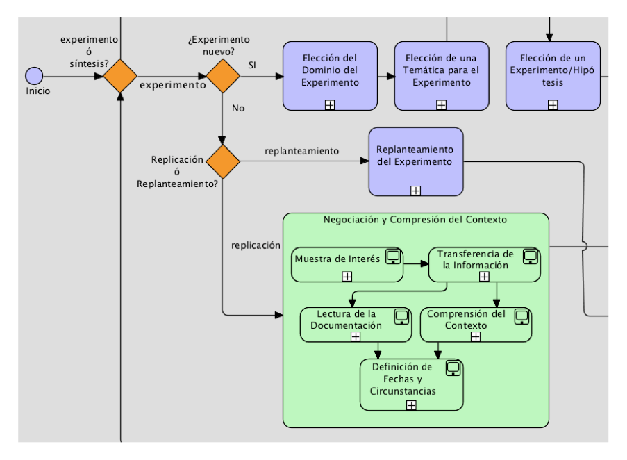
\includegraphics[width=3.2in]{images/Proccess}
	\caption{Extracto de las actividades experimentales de SE realizadas por los experimentadores del GrISE (versi�n final)}
	\label{fig-proceso-exp}
\end{figure}

Por otra parte, el proceso de entrevistas mostr� que \textit{las actividades realizadas en el GrISE difieren de un experimentador a otro; de hecho, ning�n experimentador lleva a cabo todas las actividades identificadas de la experimentaci�n en SE}{\color{blue}(17)}. Ante esto fueron consultados los miembros del GrISE, indicando que \textit{no existe una definici�n explicita para el rol que realiza cada experimentador en el grupo}{\color{blue}(30)}; de hecho, identificamos 3 grupos de actividades o roles representativos de los miembros del GrISE, a los cuales los denominaron: Research Manager (RM), Experiment Manager (EM) and Senior Experimenter (SE), los cuales en t�rminos generales se encargan de: \textit{planificar la ejecuci�n del experimento, ser el albacea de la informaci�n y gestionar la log�stica de la experimentaci�n}{\color{blue}(31)}, respectivamente.

En este punto, nos llam� la atenci�n que entre los roles identificados \textit{existen actividades experimentales que son ejecutadas por duplicado en una misma instancia experimental. Como por ejemplo: La gesti�n de la replicaci�n experimental la realizan el RM y el EM, el planteamiento del experimento lo realizan el SE y el RM}{\color{blue}(32)}. Esto ratifica la diversidad terminol�gica y operativa identificada dentro del GrISE, lo cual fue abordado puntualmente en las reuniones grupales con el prop�sito de regularizar la terminol�gica utilizada en la experimentaci�n.

\subsubsection{Formalizing de Experimental Terminology in SE}\label{subsubsec-focus-groups}
El punto de partida de la discusi�n sobre la diversidad terminol�gica y operativa de la experimentaci�n identificada en el GrISE fue el modelo conceptual (ver Figura \ref{fig-conceptos-final-revision-fuentes}) obtenido como resultado de la revisi�n del material experimental y de la literatura preferida del grupo.

Sin embargo, concretar las reuniones de discusi�n se constituy� en un verdadero problema, debido a la agenda tan apretada y variable de los miembros del GrISE, lo que caus� que la frecuencia de las reuniones sea menor y por ende el periodo de la investigaci�n debi� dilatarse considerablemente.

Las reuniones de discusi�n se caracterizaron por ser guiadas generalmente por el miembro del GrISE con mayor experiencia. Cada reuni�n tubo una duraci�n de al menos dos horas y se centraron en el debate sobre la conceptualizaci�n del proceso experimental en SE. Previo al inicio de las sesiones de discusi�n, cada miembro analiz� a detalle el modelo base, sobre el que se fueron haciendo aportes y modificaciones muy discutidas, pero finalmente al parecer consensuadas; siempre bajo la gu�a del moderador. Lo que m�s nos llam� la atenci�n en un principio fue que \textit{cada intervenci�n de los miembros del GrISE causaba que el nivel de detalle conceptual se incrementara considerablemente}{\color{blue}(23)}. No obstante, cada incremento se obten�a tras acaloradas discusiones que delataron \textit{diversidad terminol�gica incluso entre experimentadores que realizan actividades similares en una instancia experimental}{\color{blue}(24)}; pero sobre todo se observ� \textit{discrepancia conceptual sobre las actividades de experimentaci�n entre experimentadores}{\color{blue}(25)}.  

Para efectos de una abstracci�n detallada del conocimiento de los miembros del GrISE durante las sesiones de discusi�n, se utilizaron los mismos instrumentos que los utilizados en las entrevistas, en adici�n de la pizarra donde los participantes colaboraron activamente en el esbozo del modelado conceptual (ver Figura \ref{fig-conceptos-draft}). Cada sesi�n inici� con la revisi�n del producto intermedio obtenido en la reuni�n anterior, cuyo boceto fue recreado en una herramienta inform�tica y presentado al foro. El modelo base cambi� notablemente hasta llegar a un aparente modelo final (ver Figura (ver Figura \ref{fig-conceptos-exp-boseto}), \textit{el cual mostr� un amplio nivel de detalle conceptual, demostrando as� que el conocimiento m�s significativo de la experimentaci�n lo tienen los expertos}{\color{blue}(26)}. 

\begin{figure}[htbp!]
	\centering
	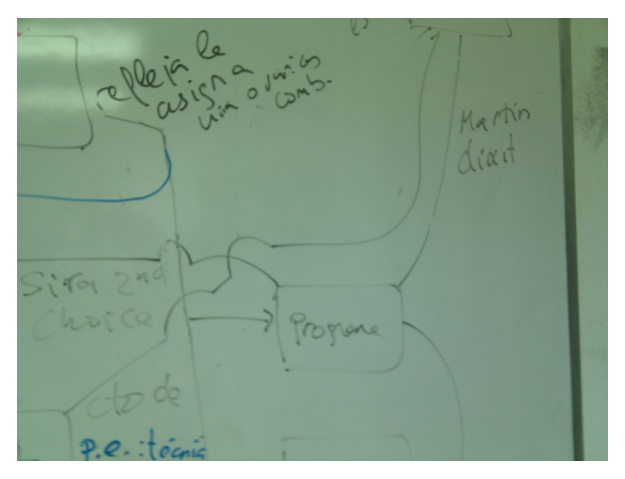
\includegraphics[width=3.4in]{images/Concept-Draft}
	\caption{Extracto del Modelo Conceptual de la Experimentaci�n en GrISE en Boceto}
	\label{fig-conceptos-draft}
\end{figure}

\begin{figure}[htbp!]
	\centering
	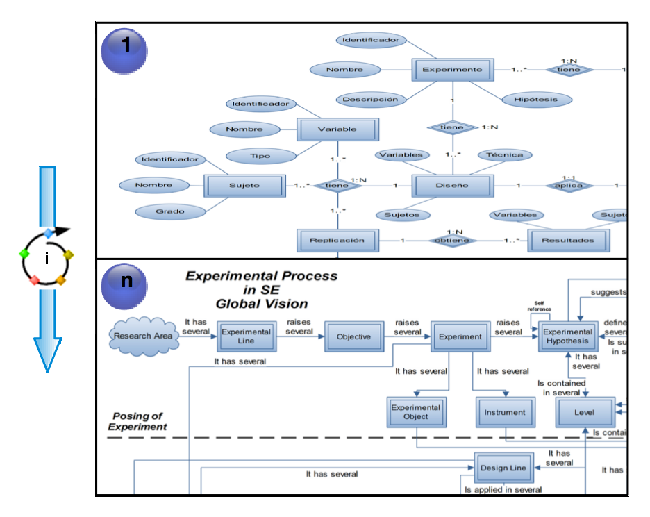
\includegraphics[width=3.4in]{images/Boseto-Concepts}
	\caption{Extracto del Modelo Conceptual de la Experimentaci�n en GrISE (versi�n final)}
	\label{fig-conceptos-exp-boseto}
\end{figure}

A pesar de que aparentemente hubo consenso en en el modelo resultante (ver Figura \ref{fig-conceptos-exp-boseto}), las acaloradas discusiones sobre los conceptos manejados y su definici�n, nos dieron pistas sobre una presunta desconformidad de algunos miembros, lo cual fue validado en las entrevistas personales que se llevaron en paralelo. El principal inconveniente argumentado por algunos miembros del GrISE sobre el modelo obtenido, fue respecto a la especialidad que tienen los miembros en fases espec�ficas del proceso, lo cual no estaba expresado en el modelo. Fue preciso entonces, iniciar un nuevo ciclo de discusiones grupales, con la particularidad de que cada experimentador expres� su conocimiento, �nicamente sobre los conceptos que maneja a trav�s de las actividades que efectivamente realiza en una instancia experimental. Este nuevo ciclo nos permiti� observar que \textit{los conceptos manejados por los experimentadores en SE obedecen a las actividades espec�ficas que realizan en una instancia experimental}{\color{blue}(18)}. Adicionalmente, se valid� \textit{la existencia de roles o perfiles de experimentadores: Experimentadores que custodian el material experimental del grupo, experimentadores que ejecutan en la pr�ctica la experimentaci�n y experimentadores que gestionan con el medio externo los nuevos experimentos y su factibilidad}{\color{blue}(33)}.

Como resultado de este nuevo ciclo de discusiones obtuvimos tres modelos conceptuales (ver Figura \ref{fig-conceptos-exp}), los cuales responden a los roles identificados durante el proceso de entrevistas.

\begin{figure}[htbp!]
	\centering
	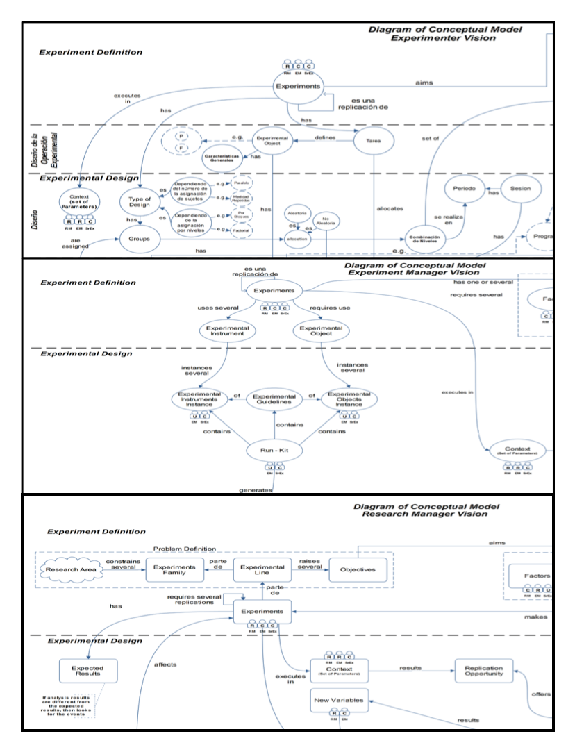
\includegraphics[width=3.4in]{Images/Concepts}
	\caption{Extracto de los Modelo Conceptuales}
	\label{fig-conceptos-exp}
\end{figure}

\subsection{Conclusions Around Findings In The Software Engineering Experimentation Process Within An Specific Research Group}
Los resultados de la investigaci�n constituyen una visi�n expl�cita de la experimentaci�n en SE dentro de un grupo de investigaci�n representativo de la comunidad de ingenier�a de software emp�rica, incluso para los mismos experimentadores que ve�an por primera vez plasmado de forma expl�cita en medios accesibles el modelo de la experimentaci�n que realizan.

Desde un inicio, llam� mucho la atenci�n la generalidad de los textos existentes y la diversidad estructural de los reportes experimentales dentro de un grupo de investigaci�n en ingenier�a de software emp�rica, lo cual no representaba una gu�a efectiva para llevar a cabo una instancia experimental en la pr�ctica. La falta de formalidad de dichos reportes experimentales impide realizar una lectura compresiva est�ndar, ya que para cada reporte es preciso descubrir su particularidad al momento de reportar; As� mismo, el uso de formatos distintos en los reportes impide identificar de forma eficiente las actividades llevadas a cabo en una instancia de experimentaci�n en SE.

Por otra parte, el formato de los archivos que contienen los datos experimentales de las distintas instancias no son est�ndar, por lo que es imposible que una persona ajena al grupo de trabajo entienda los conceptos, entidades y acr�nimos utilizados, por lo que se convierten en dependientes de las personas que los gestionan. A este respecto, se pudo percibir la necesidad de la existencia de mecanismos automatizados que guarden el v�nculo entre los experimentos y sus elementos (materiales, raw-data, dise�o, etc.), lo cual podr�a ayudar a los experimentadores a no cometer errores, dado el alto n�mero de actividades que deben cubrir.

La deficiencia en la gesti�n de la informaci�n dentro del GrISE podr�a deberse a la diversidad operativa de los experimentadores, lo que dificulta el intercambio de informaci�n, a�n incluso dentro del mismo GrISE.

Finalmente, una comunicaci�n m�s cercana con los experimentadores, permiti� encontrar detalles que generalmente no se reflejan en los reportes experimentales y que ayudaron a entender algunos resultados, conclusiones de los reportes experimentales y llevar a cabo una replicaci�n experimental. Durante las entrevistas personales mantenidas con los experimentadores se evidenci� un tipo de informaci�n impl�cita de los experimentos, la cual no es registrada en ning�n medio. Este tipo de informaci�n posiblemente proviene de la dimensi�n t�cita del conocimiento.

\section{Survey on Experimentation in Software Engineering}\label{sec-survey}

\section{Experimentation in Biotechnology}\label{sec-bio-etnography}
El estudio etnogr�fico fue realizado en tres grupos de investigaci�n (\odnote{RODRIGO: nombre grupos?}) de Ingenier�a en Biotecnolog�a de la Universidad de las Fuerzas Armadas ESPE de Ecuador. \odnote{RODRIGO: Puedes poner un poco de historia y nombrar a sus lideres, tal y como has hecho al principio de la secci�n 4?.}

La selecci�n de estos grupos se ha producido por conveniencia. No obstante, no cabe duda de que el grupo de investigaci�n es altamente competitivo a nivel internacional, como se desprende de sus publicaciones, e.g., \cite{Vizuete-2016-green-Synthesis,Villarreal-2016-Effect-Arbuscular,Kumar-2016-In-Vitro-Evaluation}. Por consiguiente, creemos que los hallazgos del estudio etnogr�fico pueden ser extrapolables a la generalidad de grupos de investigaci�n en Biotecnolog�a. 

El estudio etnogr�fico no puedo ser exactamente igual al realizado con el GrISE porque est�bamos ''contaminados'' por la experimentaci�n en SE. Por este motivo, en lugar de realizar un proceso de acercamiento progresivo, decidimos abordar aquellas actividades que nos resultaron m�s fruct�feras en GrISE: a) Estudio de la literatura preferida de los grupos de investigaci�n, b) su material experimental y, particularmente, c) el conocimiento de los experimentadores. 

Dado que nos interesa especialmente comparar la experimentaci�n en SE y Biotecnolog�a, destacaremos las caracter�sticas diferenciales de Biotecnologia mediante subrayado, al igual que hemos realizado anteriormente en la Secci�n~\ref{sec-ESE-etnography}. En algunas ocasiones, una observaci�n realizada en Biotecnolog�a arroja luz sobre la experimentaci�n en SE. Por este motivo, pueden surgir a lo largo de la exposici�n caracter�sticas espec�ficas de SE (numeradas en azul), en paralelo con las caracter�sticas espec�ficas de Biotecnolog�a (marcadas en rojo). \odnote{RODRIGO: Creo que ser�a mejor poner S1, S2, B1, B2, etc.}

\iffalse

@book{Good2012,
	Author = {Good, Phillip I and Hardin, James W},
	Publisher = {John Wiley \& Sons},
	Title = {Common errors in statistics (and how to avoid them)},
	Year = {2012}}

@book{Huck2009,
	Author = {Huck, Schuyler W},
	Publisher = {Routledge},
	Title = {Statistical misconceptions},
	Year = {2009}}

@book{Vickers2010,
	Author = {Vickers, Andrew},
	Publisher = {Addison-Wesley Longman},
	Title = {What is a P-value anyway?: 34 stories to help you actually understand statistics},
	Year = {2010}}
	
@inproceedings{Reyes2018,
  author    = {Rolando P. Reyes and
               Oscar Dieste and
               Efra{\'{\i}}n R. Fonseca C. and
               Natalia Juristo},
  title     = {Statistical errors in software engineering experiments: a preliminary
               literature review},
  booktitle = {Proceedings of the 40th International Conference on Software Engineering,
               {ICSE} 2018, Gothenburg, Sweden, May 27 - June 03, 2018},
  pages     = {1195--1206},
  year      = {2018},
  doi       = {10.1145/3180155.3180161}
}
\fi

\subsection{First approximation}\label{subsec-first-approx-biok}

La investigaci�n comenz� en noviembre de 2014. Aunque los investigadores ya hab�amos adquirido experiencia en la experimentaci�n en SE, los primeros contactos fueron dif�ciles debido al n�mero de actividades de experimentaci�n que se realizan en Biotecnolog�a, as� como a la variedad de insumos e instrumentos que se precisan dependiendo del �rea de investigaci�n. Los experimentadores en Biotecnolog�a {\color{red}(?)} \ul{no realizaban un discurso general que probablemente podr�amos comprender, sino que utilizaban terminolog�a altamente espec�fica} perteneciente a cada �rea de investigaci�n.

Los grupos en cuesti�n manejan las �reas de conocimiento de: Biotecnolog�a Humana, Biotecnolog�a Ambiental y Biotecnolog�a Vegetal. {\color{red}(?)} \ul{La especializaci�n de la investigaci�n es muy marcada respecto a lo observado en SE}. En el GrISE, el mismo grupo se dedicaba a distintas investigaciones (testing, requisitos, TDD). En cambio, en Biotecnolog�a, las �reas de investigaci�n est�n mucho m�s compartimentalizadas.

Estos grupos est�n formados esencialmente por {\color{red}(?)} \ul{un l�der (que por lo general es un investigador director de un proyecto de investigaci�n o el jefe de un laboratorio), e investigadores que son estudiantes de doctorado y master}. \odnote{RODRIGO: No hay seniors? Por qu�?}

\subsubsection{Review of preferred literature}\label{subsubsec-study-literature-case-study-2}

Los experimentadores se�alaron como textos b�sicos de Biotecnolog�a experimental a distintos libros, e.g.: \textit{Biotechnology Fundamentals} by F.A.Khan \cite{Khan-2012-Biotechnology-Fundamentals}) y \odnote{RODRIGO: poner otro libro}. Tras su revisi�n, nos sorprendi� encontrar que, al igual que en la SE, {\color{red}(15)} \ul{el proceso de experimentaci�n en Biotecnolog�a est� descrito de forma general}. As� por ejemplo \odnote{RODRIGO: Alguna an�cdota??}

No obstante, adem�s de los libros indicados anteriormente, los experimentadores disponen de {\color{red}(7)} \ul{una amplia variedad de textos, gu�as, reportes, etc. espec�ficos por tem�ticas de investigaci�n}. Por ejemplo, la \textit{Biotecnolog�a Agr�cola} by de Solaiman et al. \cite{Solaiman-2014-Mycorrhizal} describe el uso de microorganismos que se aplican a cultivos para el uso sustentable del suelo; la \textit{Biotecnolog�a Vegetal} by Bahadur et al. \cite{Bahadur-2015-Plant-Biotechnology}, se estudian todas las �micas de \textit{Arabidopsis thaliana} como modelo para el mejoramiento gen�tico de otras plantas. Esto representa una diferencia sustancial con la SE, donde {\color{blue}(?)} \ul{no existen apenas (\mbox{\cite{}\url{https://doi.org/10.1002/stvr.1486}} podr�a ser una excepci�n) textos espec�ficos de experimentaci�n por sub-�reas}, e.g., testing o requisitos. \odnote{RODRIGO: Esto lo puedes colocar en la parte de SE de la tabla~\ref{tab:comparison}}.

\odnote{RODRIGO: Sirve este texto para algo??}
\begin{tcolorbox}

No obstante, el conocimiento adquirido sobre experimentaci�n en SE, el proceso generado para su abstracci�n (particularmente aquel proveniente de la revisi�n de textos no espec�ficos de SE) y el comentario un tanto contradictorio que hac�an tambi�n los miembros de los grupos de investigaci�n sobre que \textit{en el �rea de la Biotecnolog�a se estaban aplicando propuestas alternativas de dise�o de experimentos} (e.g.: dise�os basados en el enfoque \cite{Kumar-2014-design-experiment-bioprocessing}) \textit{para la formalizaci�n del proceso experimental}{\color{red}(14)}; nos impulsaron a la realizaci�n de este estudio.

\end{tcolorbox}

Las fuentes pertenecientes a cada sub-�rea {\color{red}(1)} \ul{utilizan una terminolog�a bastante uniforme, tanto a nivel de conceptos como de procesos}, e.g.,  el \textit{Handbook} by Walker et al. \cite{Walker-2008-Handbook-Biomethods} y el libro de Ausubel et al. \cite{Ausubel-2003-Molecular-Biology} exhiben grandes similaridades en los  protocolos experimentales utilizados para el estudio de �cidos nucleicos. Por el contrario, {\color{red}(2)} \ul{encontramos diversidad (terminol�gica y operativa) entre las fuentes de sub-�reas distintas}.

\odnote{Deber�amos poner un ejemplo, y aprovechar el ejemplo para afirmar que los textos en biotecnolog�a utilizan de forma natural sus propios conceptos en la descripci�n de los protocolos. En Software, existe una separaci�n entre la terminolog�a de la parte experimental y la terminolog�a de SE.}

\subsubsection{Review of experimental material}\label{subsubsec-study-materials-case-study-2}

El material experimental propio de los grupos est� formado por sus publicaciones, datos experimentales y las denominadas libretas de laboratorio. Las libretas de laboratorio son comunes en muchas disciplinas \cite{}\url{https://www.training.nih.gov/assets/Lab_Notebook_508_(new).pdf}, aunque no en SE. Consisten en \odnote{RODRIGO: Completar}. Todos estos materiales {\color{red}(12)} \ul{resultaron ser muy espec�ficos, en consonancia con la naturaleza propia de cada �rea de conocimiento}. Por ejemplo, \odnote{RODRIGO: Alguna an�cdota??}

Durante este segundo estudio etnogr�fico, no profundizamos en la terminolog�a y operativa espec�ficas de las sub-�rea de Biotecnolog�a a las que se dedicaban los experimentadores. No era de nuestro inter�s obtener un conocimiento granular sobre conceptos ajenos a SE, ya que dif�cilmente podr�an haber sido utilizados para una comparaci�n SE vs. Biotecnolog�a. Tal y como puede comprobarse en los modelos mostrados en las Figs.~\ref{fig-proceso-exp} y \ref{fig-conceptos-exp}, los conceptos y procesos recogidos en SE poseen un alto nivel de abstracci�n. En consecuencia, los modelos de experimentaci�n en Biotecnolog�a que preparamos durante la primera aproximaci�n (v�ase, por ejemplo, la Fig.~\ref{fig-concepts-initial-bio}) fueron igualmente de alto nivel. 

De todos modos, esto no debe hacernos olvidar que \odnote{hablar de nuevo de los conceptos propios de biotecnolog�a, a los que hac�a referencia en la nota anterior}.

\odnote{RODRIGO: Entiendo que las observaciones que aparecen abajo son los aspectos del proceso experimental de Bio que te llamaron la atenci�n. Es necesario que aparezcan en el modelo de la Fig.~\ref{fig-concepts-initial-bio}. Adem�s, deber�as destacar la diferencia con SE. Puedes incluso crear nuevos hallazgos en azul. Corrige tu el texto de abajo de forma coherente con el discurso que estamos haciendo. A mi me falta contexto para hacerlo bien. Lo volver� a revisar m�s tarde, como te coment� por correo.}

\begin{tcolorbox}

Nos llam� mucho la atenci�n que, a diferencia de la SE experimental, \textit{en Biotecnolog�a consideran como fase fundamental de su proceso experimental, la generaci�n de publicaciones{\color{red}(30)}}; paralelamente, \textit{gestionan de forma �gil la investigaci�n a nivel de documentaci�n y recursos utilizados; particularmente los recursos humanos, econ�micos y legales}{\color{red}(13)}.

Otra caracter�stica que nos pareci� peculiar de los grupos de investigaci�n estudiados, fue que \textit{los reportes experimentales son similares en formato y centran su discurso en los resultados generales de cada ensayo (experimento), los cuales se basan en la comparaci�n de tratamientos individuales}{\color{red}(29)}; as� mismo, \textit{encontramos indicios de que las actividades de experimentaci�n realizadas en Biotecnolog�a constituyen la estructura de los reportes experimentales que publican}{\color{red}(32)}.

Lo mismo ocurri� con los datos experimentales, dado que su preservaci�n no es muy importante en estos grupo de investigaci�n; de hecho, \textit{los datos obtenidos en las instancias experimentales son utilizados hasta su reporte, luego de lo cual son almacenados en repositorios experimentales locales o p�blicos para futuros re an�lisis o s�ntesis de resultados, o simplemente son descartado}{\color{red}(20)}. Estas caracter�sticas influyeron negativamente, sobredimensionando en un inicio nuestra percepci�n sobre la complejidad de la investigaci�n por realizar.

Otro de los factores que posiblemente ha incidido en la formalidad de los procesos experimentales estudiados, es \textit{el gran volumen de informaci�n que se maneja en estos grupos de investigaci�n, lo cual ha obligado a que el formato de los contenedores de datos experimentales sea est�ndar (hojas excel o repositorios)}{\color{red}(10)}, \textit{lo que facilita el acceso y utilizaci�n a otros grupos que investigan en la misma tem�tica}{\color{red}(11)}. De forma similar \textit{la formalidad operativa del proceso ha debido materializarse para mejorar la efectividad en la gesti�n e intercambio de la informaci�n{\color{red}(19)}}. Todo esto se ha visto reflejado en la \textit{construcci�n de mecanismos automatizados que guarden el v�nculo entre los experimentos y sus elementos (materiales, raw-data, dise�o, etc.) para ayudar a los experimentadores, entre otras cosas, a gestionar f�cilmente los datos experimentales}{\color{red}(22)}.
 
\end{tcolorbox}

\odnote{Hay una contradicci�n entre el ''desconocimiento'' afirmado aqu� y la ''falta de inter�s en obtener conocimiento granular'' indicado un poco m�s arriba.}

El desconocimiento por parte de los investigadores de las �reas de conocimiento de Biotecnolog�a limitaron los resultados de esta primera fase a la obtenci�n de un modelo gen�rico muy b�sico de la experimentaci�n en Biotecnolog�a. Para profundizar, aplicamos la misma estrategia que en SE y entrevistamos a los miembros de los grupos de investigaci�n objeto de estudio.
  
\subsection{Understanding the Experimental Process in Detail}\label{subse-experimental-process-biotech}

Realizamos las entrevistas siguiendo la misma estrategia que en GrISE \odnote{????}. \odnote{RODRIGO: El p�rrafo que sigue es oscuro. No entiendo si las entrevistas han sido individuales o grupales, si ha habido cambios en el medio del proceso, ni en qu� consiste la variaci�n en la t�cnica de abstracci�n.}

\begin{tcolorbox}

Sin embargo, la diversidad terminol�gica y operativa de la experimentaci�n entre �reas del conocimiento dificult� identificar un �nico proceso formal. Por lo tanto, nos vimos obligados a variar un tanto la t�cnica de abstracci�n del conocimiento en los acercamientos planificados con los miembros de los grupos.

\end{tcolorbox}

\subsubsection{Interviews with biotechnology experimenters}

Utilizamos el mismo cuestionario de preguntas abiertas, recolecci�n de datos, y an�lisis de protocolos que en el estudio etnogr�fico realizado con los experimentadores de SE. Los esbozos realizados por algunos experimentadores en papel o en la pizarra (ver Fig.~\ref{fig-proc-exp-esbozo}) y el relato escrito abstra�do de las entrevistas sobre las actividades que realizan en el proceso experimental, permiti� ir sintetizando en un �nico modelo, que fue digitalizado utilizando software especializado. En cada sesi�n fue validado el modelo por los experimentadores, hasta obtener un modelo final (ver Fig.~\ref{fig-proceso-exp-final}). 

\begin{figure}[htbp!]
	\centering
	\includegraphics[width=3.2in]{Images/Outline-Process}
	\caption{Esbozo de las Actividades Experimentales de Biotecnolog�a}
	\label{fig-proc-exp-esbozo}
\end{figure}

La primera diferencia significativa que percibimos respecto a la experimentaci�n en SE fue que {\color{red}(17)} \ul{el protocolo experimental en Biotecnolog�a es formal y detallado}. Por ejemplo, \odnote{RODRIGO: Poner alguna evidencia que justifique por qu� es as�. Quiz�s puedas describir el proceso un poco, haciendo referencia a la figura \ref{fig-proceso-exp-final}.}

\odnote{Debemos usar el t�rmino ''protocolo'' o ''proceso''??}

El protocolo experimental en Biotecnolog�a no s�lo est� bien definido, sino que tambi�n {\color{red}(26)} \ul{est�n bien definidos los roles de cada experimentador dentro del protocolo experimental}, lo que {\color{red}(25)} \ul{no permite que exista solapamiento de actividades entre los experimentadores}. Por ejemplo, el \textit{Biometrista} se encarga del an�lisis de datos, mientras que \odnote{RODRIGO: Completar. Qu� ventajas tiene la definici�n de roles? Una mejor ejecuci�n del protocolo? Los roles son comparables a los de SE? Parece que no. Qu� diferencias existen?}.

\odnote{He puesto en las conclusiones de la secci�n 4 que la compartimentalizaci�n de los roles es un problema. No lo parece, visto lo que ocurre aqu�.}

\odnote{Falta algo. Quiz�s referido a las salidas del proceso experimental? Quiz�s te sirva el texto siguiente:}

\begin{tcolorbox}

Sin embargo, \textit{la formalidad que se maneja en los reportes experimentales de estas �reas permite identificar f�cilmente las actividades llevadas a cabo en su proceso experimental}{\color{red}(33)}, \textit{lo que permiten replicar sin mayor complicaci�n los estudios realizados}{\color{red}(23)}; de hecho, \textit{tal es la claridad de los reportes que sin ser conocedores o expertos en el �rea, se puede entender claramente sus resultados, conclusiones y discusi�n}{\color{red}(21)}.

\end{tcolorbox}

\odnote{RODRIGO: Quiz�s puedas mover aqu� texto del cuadro de la seccion 6.1.2, probablemente los problemas 29 y 32.}

\odnote{Rodrigo: Entonces, deber�a haber 3 modelos de conceptos, y 3 modelos de procesos, no es as�??}

Result� imposible crear un modelo �nico que acomodara los conceptos y actividades empleados en cada sub-�rea de conocimiento. Esto era previsible, ya que las distintas sub-�reas manejaban distinta terminolog�a. Aun as�, nos planteamos realizar una serie de workshops, al igual que hicimos en SE, para verificar si realmente crear un modelo �nico era imposible, o por el contrario era un problema aparente que surg�a por el hecho de que las entrevistas realizadas en esta fase de la investigaci�n eran individuales.

\subsubsection{Workshops}

\odnote{RODRIGO: Tendr�s que clarificar qu� modelos se han obtenido en las distintas fases de la investigaci�n etnogr�fica.}

Las sesiones de discusi�n tuvieron como prop�sito armonizar la terminolog�a identificada en las �reas de conocimiento estudiadas. \odnote{RODRIGO: Qui�nes participaron, cu�ntos workshops, cu�nto tiempo??}. El proceso inici� con el debate sobre el modelo conceptual resultante de la review of preferred literature (ver Fig.~\ref{fig-concepts-initial-bio}). De cada sesi�n de discusi�n se obtuvo un producto intermedio, el cual fue validado y depurado por el grupo en la siguiente instancia, hasta obtener un producto final (ver Fig.~\ref{fig-concepts-final-bio}).

\odnote{Rodrigo: Termina esto tu. A mi me falta contexto.}

\begin{tcolorbox}

Las distintas sesiones de discusi�n nos mostraron que \textit{la cantidad de conceptos que intervienen en el proceso de experimentaci�n en Biotecnolog�a es alta}{\color{red}(18)}. Aunque no fue tan intenso el debate, las discusiones m�s importantes se centraron en los conceptos que difer�an de una a otra �rea de conocimiento, constat�ndose que \textit{los experimentadores de un mismo grupo de investigaci�n en Biotecnolog�a utilizan una terminolog�a com�n para comunicarse}{\color{red}(3)}; adicionalmente, se observ� que \textit{los conceptos manejados por los experimentadores en Biotecnolog�a corresponden a las actividades espec�ficas del rol que cumplen en cada proceso experimental}{\color{red}(27)}. La baja intensidad en las discusiones nos permiti� constatar que \textit{cada experimentador tiene una especialidad y por ende fue relativamente sencilla la conformaci�n del modelo conceptual}{\color{red}(28)}.

\end{tcolorbox}

\odnote{No me queda claro qu� modelos se elaboraron finalmente, ni si se consigui� un modelo conjunto. Si se consigui� un modelo conjunto, tuvo alg�n coste (ej: perdida de detalle)?}

\subsection{Conclusions}

Al igual que en el caso de SE, la investigaci�n etnogr�fica termin� al finalizar los workshops. En esta ocasi�n, la etnograf�a no tuvo un car�cter tan marcado de observaci�n participativa, pero a�n as� la interacci�n con los grupos de investigaci�n en Biotecnolog�a tuvo una larga duraci�n en el tiempo (XXX meses) e implic� establecer relaciones estrechas con los investigadores. En la Secci�n~\ref{sec-discussion-conclusions} realizaremos una comparaci�n expl�cita entre la experimentaci�n en SE y Biotecnolog�a, pero antes de ello resumimos los principales hallazgos obtenidos en esta segunda investigaci�n etnogr�fica:

\odnote{RODRIGO: Completar.}

\begin{itemize}

\item Los textos gen�ricos de Biotecnolog�a no representan una gu�a efectiva para llevar a cabo experimentos en la pr�ctica en �reas espec�ficas de la Biotecnolog�a

\end{itemize}





\section{Threats to Validity}\label{sec-threats}
\subsection{Threats to validity}
El procedimiento planteado en la metodolog�a en conjunto contribuye positivamente con la validez de la investigaci�n, el cual se basa en:
\begin{itemize}
  \item Muestras representativas del universo bajo estudio
  \item Proceso exhaustivo de revisi�n de las fuentes de informaci�n
  \item Verificaci�n de los resultados en cada iteraci�n de revisi�n de las fuentes de informaci�n
  \item Validaci�n cruzada de informaci�n
\end{itemize}

Los inconvenientes presentados por el uso de las diferentes t�cnicas e instrumentos fueron minimizados gracias a su combinaci�n en cada iteraci�n. Por ejemplo, los vac�os del audio fueron complementados por el video, las fotograf�as y los esbozos de los experimentadores y viceversa.

\section{Discussion}\label{sec-discussion}

\odnote{Cada una de las cosas que se�alamos en las etnograf�as ser�n ''observaciones''. Se convierten en ''hallazgos'' en la discusi�n.}

\odnote{Para Oscar: Recordemos hablar de las correlaciones vs. causalidades en las conclusiones. Dicho de otro modo: nuestros hallazgos deber�an ser referendados por otros estudios.} 

\vspace{5mm}

\color{purple}

Respecto a los modelos: no nos preocupa demasiado ---> referirse a la publicaci\'on del IJSEKE

\color{black}

\color{red}

Some of our findings may not be surprising, but as argued by Torchiano and
Ricca, reporting on the reality may not always offer surprising insights (Torchiano
and Ricca, 2013). Yet, empirical evidence offers a scientific basis to better understand 
reality and advance the aspects under study \cite{torchiano2013six}

\color{black}

Esta investigaci�n tiene como objetivo comparar el modo en que se realizan experimentos en IS y en otra disciplina experimental parecida, en concreto, la Ingenier�a en Biotecnolog�a. Esta comparaci�n se basa en una premisa que no hemos hecho expl�cita, pero que es f�cilmente reconocible: las disciplinas experimentales asentadas poseen ''mejores'' pr�cticas experimentales que la IS. En consecuencia, averiguar las diferencias entre la experimentaci�n en IS y otras disciplinas podr�a sugerir alternativas de mejora.

No entraremos a discutir si la premisa anterior es cierta o no. Por una parte, cualquier alternativa de mejora que podamos sugerir no puede ser asumidas de forma acr�tica en IS; su introducci�n requerir�a un proceso de validaci�n que pondr�a de manifiesto fortalezas y debilidades. Por otra parte, la mera comparaci�n de procesos experimentales, independientemente de su importancia epistemol�gica, resultar� sin duda ilustrativa a los investigadores de IS. Lograr esto �ltimo, i.e.:, reflexionar acerca del proceso experimental en IS, es lo que realmente deseamos alcanzar.

\footnotesize
% Please add the following required packages to your document preamble:
% \usepackage{multirow}
% \usepackage{lscape}
% \usepackage{longtable}
% Note: It may be necessary to compile the document several times to get a multi-page table to line up properly
\begin{landscape}
\begin{longtable}[c]{|p{0.09\textwidth}|p{0.02\textwidth}|p{0.35\textwidth}|p{0.35\textwidth}|p{0.02\textwidth}|p{0.3\textwidth}|}
\caption{Hallazos obtenidos en los estudios etnogr�ficos. \odnote{RODRIGO: intenta que los c�digos de las observaciones vayan en secuencia dentro de cada ''bloque''}}
\label{tab:comparison}\\
\hline
\textbf{Type}                          & (S\#)              & Observaciones del estudio en SE                                                                                                                                                                                                                     & Observaciones del estudio en Biotecnolog�a                                                                                                                                        & (B\#)               & Hallazgos                                                                                                                                                                                                                                                    \\ \hline
\endfirsthead
%
\multicolumn{6}{c}%
{{\bfseries Table \thetable\ continued from previous page}} \\
\hline
\textbf{Type}                          & (S\#)              & Observaciones del estudio en SE                                                                                                                                                                                                                     & Observaciones del estudio en Biotecnolog�a                                                                                                                                        & (B\#)               & Hallazgos                                                                                                                                                                                                                                                    \\ \hline
\endhead
%
\multirow{4}{*}{\textbf{Fuentes}}      & 5                  & La carencia de textos de referencia es un aspecto caracter�stico de la experimentaci�n en SE.                                                                                                                                                       & \multirow{2}{0.35\textwidth}{La diversidad de libros de texto experimentales en Biotecnolog�a es notable.}                                                                                     & \multirow{2}{*}{2}  & \multirow{2}{0.3\textwidth}{La disponibilidad de textos de referencia en Biotecnologia es mucho mayor que en ESE.}                                                                                                                                                        \\ \cline{2-3}
                                       & 1                  & Las fuentes b�sicas para su proceso de experimentaci�n a los libros by \cite{Wohlin2000} and \cite{Juristo2001}.                                                                    &                                                                                                                                                                                   &                     &                                                                                                                                                                                                                                                              \\ \cline{2-6} 
                                       & 2                  & En el RGUS tambi�n se utilizan como fuentes b�sicas ciertos reportes o art�culos espec�ficos.                                                                                                                                                       & \multirow{2}{0.35\textwidth}{Los experimentadores disponen de una amplia variedad de textos, gu�as, reportes, etc. espec�ficos por tem�tica de investigaci�n}                                  & \multirow{2}{*}{4}  & \multirow{2}{0.3\textwidth}{La disponibilidad de materiales especificos por �rea en ESE es pr�cticamente inexistente.}                                                                                                                                                    \\ \cline{2-3}
                                       & 31                 & No existen apenas textos espec�ficos de experimentaci�n por sub-�reas, e.g., testing o requisitos; el trabajo de \cite{Arcuri-2014-statistical-tests} es una de las pocas excepciones existentes.                                 &                                                                                                                                                                                   &                     &                                                                                                                                                                                                                                                              \\ \hline
\multirow{7}{*}{\textbf{Terminolog�a}} & \multirow{2}{*}{3} & \multirow{2}{0.35\textwidth}{A pesar de las escasas fuentes bibliogr�ficas sobre ESE, la diversidad terminol�gica con que dichas fuentes se refer�an a actividades similares del proceso de experimentaci�n es vasta.}                                           & Las fuentes pertenecientes a cada tem�tica utilizan una terminolog�a bastante uniforme, tanto a nivel de conceptos como de procesos.                                              & 5                   & \multirow{4}{0.3\textwidth}{Los conceptos experimentales m�s generales, e.g., objetivo, hip�tesis,variable respuesta, etc., son similares en ESE y Biotecnolog�a, aunque no exista coincidencia debido a las respectivas tradiciones de cada disciplina.}                 \\ \cline{4-5}
                                       &                    &                                                                                                                                                                                                                                                     & Encontramos diversidad (terminol�gica y operativa) entre las fuentes de tem�ticas distintas.                                                                                      & 6                   &                                                                                                                                                                                                                                                              \\ \cline{2-5}
                                       & \multirow{2}{*}{4} & \multirow{2}{0.35\textwidth}{No est� claro si los distintos autores conciben exactamente de la misma forma a las actividades del proceso de experimentaci�n.}                                                                                                    & El proceso de experimentaci�n en Biotecnolog�a est� descrito de forma bastante general                                                                                            & 3                   &                                                                                                                                                                                                                                                              \\ \cline{4-5}
                                       &                    &                                                                                                                                                                                                                                                     & A nivel de la literatura preferida, tanto los conceptos como los procesos son generales                                                                                           & 8                   &                                                                                                                                                                                                                                                              \\ \cline{2-6} 
                                       & 13                 & Los reportes sufr�an de incluso mayor diversidad terminol�gica que los libros de referencia.                                                                                                                                                        & Los reportes experimentales son similares en formato y terminolog�a dentro de cada �rea.                                                                                          & 10                  & \multirow{3}{0.3\textwidth}{Aunque en ESE no existe una diferenciaci�n de la investigaci�n experimental por �reas, la diversidad de m�todos utilizados aparece reflejada en los materiales y reportes experimentales.}                                                    \\ \cline{2-5}
                                       & 16                 & El tipo y nivel de detalle de los materiales experimentales estaba en relaci�n a las tareas que los sujetos deb�an realizar.                                                                                                                        & \multirow{2}{0.35\textwidth}{Los conceptos, actividades y materiales experimentales de cada tem�tica de investigaci�n resultaron ser muy espec�ficos}                                          & \multirow{2}{*}{9}  &                                                                                                                                                                                                                                                              \\ \cline{2-3}
                                       & 30                 & Los conceptos manejados por los experimentadores en SE obedecen a las actividades espec�ficas que realizan en una instancia experimental.                                                                                                           &                                                                                                                                                                                   &                     &                                                                                                                                                                                                                                                              \\ \hline
\multirow{3}{*}{\textbf{Educaci�n}}    & 28                 & La diversidad terminol�gica entre experimentadores parece deberse al tipo de formaci�n que cada experimentador ha recibido.                                                                                                                         & \multirow{2}{0.35\textwidth}{Las discusiones m�s importantes se centraron en los conceptos que difer�an de una a otra tem�tica; dentro de cada �rea, los conceptos est�n muy estadarizados.}   & \multirow{2}{*}{22} & \multirow{2}{0.3\textwidth}{La formaci�n de los investigadores en ESE es muy heterog�nea en comparaci�n a la formaci�n en Biotecnolog�a.}                                                                                                                                 \\ \cline{2-3}
                                       & 29                 & Dado que la terminolog�a en cada una de estas tradiciones difiere, la diversidad terminol�gica era una consecuencia inevitable.                                                                                                                     &                                                                                                                                                                                   &                     &                                                                                                                                                                                                                                                              \\ \cline{2-6} 
                                       & 11                 & El RGUS ha realizado distintas familias de experimentos.                                                                                                                                                                                            & La especializaci�n de la investigaci�n es muy marcada respecto a lo observado en SE.                                                                                              & 1                   & Los grupos de investigaci�n en Biotecnolog�a realizan experimentos en �reas muy concretas, frente a los grupos de ESE que son m�s generalistas.                                                                                                               \\ \hline
\multirow{9}{*}{\textbf{Operaci�n}}    & 14                 & La carencia de una gu�a detallada de las actividades que se realizan en la pr�ctica antes, durante y despu�s de la experimentaci�n.                                                                                                                 & \multirow{3}{0.35\textwidth}{El proceso experimental en Biotecnolog�a es formal y detallado}                                                                                                   & \multirow{3}{*}{14} & \multirow{5}{0.3\textwidth}{El proceso experimental en Biotecnolog�a puede describirse como una caja blanca. Por el contrario, en ESE, el proceso experimental representa en gran medida una caja negra que depende fuertemente del investigador que lo ejecute.}         \\ \cline{2-3}
                                       & 9                  & Las actividades, de la mano del material experimental, han ido evolucionando y mejorando con el tiempo.                                                                                                                                             &                                                                                                                                                                                   &                     &                                                                                                                                                                                                                                                              \\ \cline{2-3}
                                       & 10                 & Los documentos del RGUS se caracterizan por mostrar una descripci�n general de las actividades a ser realizadas en el experimento, pero no proporcionan una gu�a clara sobre el orden de ejecuci�n y relaci�n entre las actividades experimentales. &                                                                                                                                                                                   &                     &                                                                                                                                                                                                                                                              \\ \cline{2-5}
                                       & 23                 & Los textos sobre experimentaci�n en SE existentes y el material experimental del grupo est�n lejos de mostrar el trabajo real que implica la experimentaci�n en la pr�ctica.                                                                        & Las libretas de laboratorio consisten en un registro completo de un experimento                                                                                                   & 7                   &                                                                                                                                                                                                                                                              \\ \cline{2-5}
                                       & 22                 & La existencia de un profundo conocimiento t�cito, particular de cada experimentador.                                                                                                                                                                & Los protocolos dentro de cada �rea de Biotecnolog�a son muy similares entre s�.                                                                                                   & 19                  &                                                                                                                                                                                                                                                              \\ \cline{2-6} 
                                       & 6                  & No existe una pol�tica de gesti�n del material experimental.                                                                                                                                                                                        & Gestionan de forma �gil la investigaci�n a nivel de documentaci�n y recursos utilizados; particularmente los recursos humanos, econ�micos y legales.                              & 13                  & \multirow{3}{0.3\textwidth}{En Biotecnolog�a, se realiza una gesti�n espec�fica de los materiales experimentales. En ESE, la gesti�n depende en gran medida de cada investigador particular.}                                                                             \\ \cline{2-5}
                                       & 8                  & Algunas publicaciones incluso podr�an no haber estado accesibles, de no existir librer�as digitales.                                                                                                                                                & En Biotecnolog�a consideran como fase fundamental de su proceso experimental, la generaci�n de publicaciones.                                                                     & 12                  &                                                                                                                                                                                                                                                              \\ \cline{2-5}
                                       & 7                  & La ubicaci�n y formato de los raw data son conocidos �nicamente por la persona que los gestiona.                                                                                                                                                    & Los contenedores de datos experimentales (ya sean hojas Excel o repositorios) est�n razonablemente estandarizados.                                                                & 11                  &                                                                                                                                                                                                                                                              \\ \cline{2-6} 
                                       & 12                 & Existe una diversidad de aproximaciones y enfoques sobre la realizaci�n de experimentos, dependiendo de la familia y el investigador que los plantee.                                                                                               & El protocolo experimental aplicado depende del prop�sito de la investigaci�n y de las caracter�sticas de los objetos experimentales                                               & 15                  & Los protocolos experimentales dependen del �rea de investigaci�n tanto en Biotecnolog�a como en ESE (en ESE, el investigador tambi�n representa una importante fuente de variabilidad).                                                                        \\ \hline
\multirow{4}{*}{\textbf{Roles}}        & 24                 & Dentro de un grupo de investigaci�n las responsabilidades se distribuyen en diversos roles.                                                                                                                                                         & \multirow{2}{0.35\textwidth}{Los roles de cada experimentador dentro del proceso de un experimento est�n bien definidos.}                                                                      & \multirow{2}{*}{20} & \multirow{2}{0.3\textwidth}{En Biotecnolog�a, los experimentadores poseen roles bien definidos. En ESE, el mismo experimenador puede desempe�ar varios roles al mismo tiempo, o distintos roles en distintos experimentos.}                                               \\ \cline{2-3}
                                       & 25                 & No existe una asignaci�n explicita de roles a personas.                                                                                                                                                                                             &                                                                                                                                                                                   &                     &                                                                                                                                                                                                                                                              \\ \cline{2-6} 
                                       & 26                 & Existen actividades experimentales que son ejecutadas por distintos roles dentro de cada familia de experimentos.                                                                                                                                   & No exista solapamiento de actividades entre los experimentadores.                                                                                                                 & 21                  & Las actividades de los roles no est�n bien definidas en ESE.                                                                                                                                                                                                  \\ \cline{2-6} 
                                       & 27                 & Existencia de diversidad terminol�gica incluso entre experimentadores que realizan actividades similares dentro de una misma familia de experimentos.                                                                                               & Los conceptos manejados por los experimentadores corresponden a las actividades espec�ficas del rol que cumplen en un experimento.                                                & 23                  & La diversidad terminol�gica en ESE se ve empeorada debido a que distintos experimentadores, con distinta formaci�n y conocimiento t�cito, pueden desempe�ar el mismo rol.                                                                                     \\ \hline
\multirow{6}{*}{\textbf{Replicaci�n}}  & 20                 & No existen gu�as claras que permita realizar una replicaci�n literal, externa e independiente del experimento original.                                                                                                                             & La formalidad del proceso experimental facilita la realizaci�n de replicaciones experimentales.                                                                                   & 18                  & \multirow{3}{0.3\textwidth}{La formalidad y visibilidad del proceso en Biotecnolog�a permite una sencilla realizaci�n de las replicaciones experimentales. En ESE es necesaria el soporte de los investigadores originales para llevar a cabo una replicaci�n con �xito.} \\ \cline{2-5}
                                       & 15                 & Para planificar la replicaci�n fue necesario contar con la participaci�n directa de los experimentadores que realizaron el experimento original.                                                                                                    & \multirow{2}{0.35\textwidth}{Es posible entender gran parte de los reportes experimentales, e.g., resultados, conclusiones y discusi�n sin ser conocedores del �rea o requerir ayuda externa.} & \multirow{2}{*}{17} &                                                                                                                                                                                                                                                              \\ \cline{2-3}
                                       & 21                 & Es necesaria la presencia de los experimentadores originales durante buena parte del proceso para que los resultados del baseline experiment y la replicaci�n sean comparables.                                                                     &                                                                                                                                                                                   &                     &                                                                                                                                                                                                                                                              \\ \cline{2-6} 
                                       & 17                 & La primera fase de la medici�n del experimento carec�a de sistematicidad, aunque trat�ndose de un experimento espec�fico podr�a ser algo particular de esta �rea experimental.                                                                      & \multirow{3}{0.35\textwidth}{Ciertas actividades, como pueden ser la medici�n o el an�lisis, parecen ser comunes en distintas disciplinas experimentales.}                                      & \multirow{3}{*}{16} & \multirow{3}{0.3\textwidth}{Ciertas actividades, como pueden ser la medici�n o el an�lisis, parecen ser entre comunes en distintas areas dentro de la misma disciplina, as� como entre disciplinas experimentales.}                                                      \\ \cline{2-3}
                                       & 18                 & La SE (como la Psicolog�a) trabajan con constructos no observables (e.g., calidad) que se operacionalizan de modo no-est�ndar, en lugar de m�tricas bien definidas como ocurre en otras �reas (e.g., longitud en F�sica).                           &                                                                                                                                                                                   &                     &                                                                                                                                                                                                                                                              \\ \cline{2-3}
                                       & 19                 & Tanto el an�lisis como el reporte fueron sencillos de realizar, lo que al parecer se debe a que estas actividades son m�s generales que las indicadas anteriormente.                                                                                &                                                                                                                                                                                   &                     &                                                                                                                                                                                                                                                              \\ \hline
\end{longtable}
\end{landscape}
\normalsize

Los observaciones realizadas en este estudio se reportan en la Table~\ref{tab:comparison}, agrupados por tipo. Esta agrupaci�n es la misma que hemos venido usando en las conclusiones de las etnograf�as de IS y Biotecnolog�a (Secciones~\ref{sec-ESE-etnography-conclusion} y \ref{sec-Bio-etnography-conclusion}), aunque all� el nivel de detalle era mucho menor. La Table~\ref{tab:comparison} no s�lo indica todas las observaciones importantes realizadas, sino tambi�n los hallazgos que surgen de la comparaci�n de las caracter�sticas de la IS y la Biotecnolog�a es mucho mayor, y que pasaremos a comentar a continuaci�n.

Respecto a las fuentes utilizadas en IS y en Biotecnolog�a, hemos constatado que existe una mayor variedad de textos de referencia en Biotecnolog�a que en IS. Esto era esperable, dado que la investigaci�n experimental en IS representa s�lo una fracci�n de la investigaci�n realizada en Biotecnolog�a. A modo de ejemplo, a nivel mundial se han gastado \textcolor{red}{\$XXX} \odnote{buscar referencia} en investigaci�n Biotecnol�gica, la mayor�a probablemente de car�cter experimental. Aunque no disponemos de datos, la IS experimental queda sin duda muy por detr�s. Otro hallazgo relevante es que la mayor�a del las fuentes utilizadas en IS son generalistas. Apenas existen materiales espec�ficos por �rea de investigaci�n en IS, e.g., testing \cite{Paper de Lionel briand}. El problema de la falta de especializaci�n en IS es probablemente relevante y aparecer� de forma continuada a lo largo de la discusi�n.

Las diferencias terminol�gicas entre IS y Biotecnolog�a son relativamente escasas cuando se aborda la experimentaci�n a alto nivel (discutiendo acerca de factores, niveles, variables respuesta, etc.). Se podr�a afirmar que los \textit{procesos} experimentales (ver Secci�n~\ref{sec-background}) de ambas disciplinas son razonablemente equivalentes. La situaci�n cambia a nivel de tem�tica o �rea, donde la importancia del proceso se ve desplazada por el detalle de los \textit{protocolos y materiales experimentales} (ver de nuevo la Secci�n~\ref{sec:background}). En este caso, existen profundas diferencias terminol�gicas entre distintas �reas de la Biotenolog�a. En IS, dichas diferencias parece que tambi�n est�n presentes, pero la falta de especializaci�n en IS no permite observar dichas diferencias con claridad.

Otro aspecto diferencial entre la IS y la Biotecnolog�a, tambi�n relacionado con la especializaci�n, es la formaci�n y aplicaci�n del conocimiento cient�fico-t�cnico. Los investigadores en Biotecnolog�a tienen una muy formaci�n homog�nea comparada con la de los investigadores en IS. Del mismo modo, la investigaci�n en Biotecnolog�a es especializada, mientras que en IS es generalista, i.e., el mismo grupo de IS realiza experimentos en distintas �reas. Esto es notable, ya que la especializaci�n no est� relacionada con el tama�o de los grupos: los grupos de investigaci�n en Biotecnolog�a son comparables en tama�o, o incluso m�s grandes, que los grupos de IS.

En Biotecnolog�a, existe una gran visibilidad en las operaciones realizadas durante la ejecuci�n de un experimento. Los protocolos y materiales son uniformes dentro de cada �rea, utilizan una terminolog�a uniforme (como se ha indicado anteriormente), y por lo tanto son independientes del investigador que los implementa. En IS, los protocolos y materiales dependen fuertemente del investigador, y por lo tanto la cooperaci�n con terceros no es sencilla o, por lo menos, inmediata. La operaci�n se ve beneficiada adicionalmente en Biotecnolog�a gracias a la existencia de una pol�tica de gesti�n de materiales y datos experimentales. De nuevo, en IS dicha pol�tica depende en gran medida de cada investigador.

No obstante, la operaci�n en Biotecnolog�a no se ve favorecida �nicamente por la estandarizaci�n de protocolos y m�todos. El recurso humano juega un papel primordial. En Biotecnolog�a, los experimentadores poseen no s�lo una especializaci�n a nivel de tem�tica o �rea, sino tambi�n en lo tocante a los conocimientos o pericias que ponen en juego a la hora de realizar un experimento. Es lo que hemos denominado \textit{roles}. En Biotecnolog�a, cada experimentador tiene normalmente un rol bien definido. En IS existen roles, pero ni est�n bien definidos, ni existe una asignaci�n consistente de roles a investigadores. El mismo experimentador de IS puede desempe�ar distintos roles en distintos experimentos.

Finalmente, la formalidad del proceso y protocolos experimentales en Biotecnolog�a permite realizar de forma relativamente sencilla replicaciones experimentales. En IS es necesaria el soporte de los investigadores originales para replicar un experimento, con pocas excepciones, e.g., la medici�n o el an�lisis.

\odnote{RODRI: Cuando la tabla est� finalizada, copiar aqu�}

\section{Conclusions}\label{sec-discussion-conclusions}

El estudio etnogr\'afico realizado muestra que existen diferencias entre el proceso experimental, tal y como es concebido en la teor\'ia, y su aplicaci\'on pr\'actica. Las descripciones que los experimentadores hacemos de los experimentos deben mucho al modo en que los reportamos, pero el reporte es s\'olo una conceptualizaci\'on final del proceso investigativo, que muchas veces diverge del modo en que los experimentos fueron realmente dise\~nados y ejecutados \cite{medawar1990scientific}. Creemos que muchos experimentadores de la ESE se ver\'an reconocidos en las observaciones que hemos realizado, aunque los detalles concretos pueden variar dependiendo del grupo de investigaci\'on involucrado.

Las conclusiones del estudio arrojan luz sobre varios aspectos relevantes de la ESE. El primero, y m\'as sencillo, es el tema de la educaci\'on de los investigadores. El amateurismo provoca problemas de comunicaci\'on, lo que a su vez complica la replicaci\'on experimental.�No hemos sido los primeros en identificar este problema \odnote{RODRIGO: necesito citas}\odnote{Poner citas del paper de las entrevistas de Rolando} y est\'a claro que hay que solucionarlo. Sin embargo, creemos que la soluci\'on no pasa simplemente por establecer un curriculum; es necesario algo m\'as.

Dos cosas que hemos aprendido durante la investigaci\'on son que: 1) Es poco probable que se pueda llegar a un acuerdo dentro de la comunidad ESE acerca de un proceso experimental general, ya que 2) cada \'area de investigaci\'on tiene caracter\'isticas particulares. Por poner un ejemplo, aunque superficialmente un experimento de \textit{mutation testing} es similar a un experimento de \textit{requirements elicitation}, las claves para entender dichos experimentos podr\'ian est\'an en el modo de generaci\'n de los mutantes o en los modelos conceptuales del dominio del problema, respectivamente. Sin formaci\'on espec\'ifica, los experimentadores en testing no van a entender mejor el experimento de elicitaci\'on, y viceversa, por mucho que etiquetemos dichos conceptos como ''objetos experimentales.'' Y lo que es peor; una vez comprendidos dichos conceptos, la etiqueta ''objeto experimental'' puede resultar excesivamente general, y por lo tanto de poco valor para el experimentador conocedor del \'area de investigaci\'on.

Por este motivo, creemos que es mucho m�s importante abordar la educaci\'on en experimentaci�n dentro �reas concretas, no a nivel general. Cada \'area deber\'ia desarrollar su terminolog\'ia y procedimientos propios. En cierto sentido, esto ya est\'a ocurriendo. A principios de los a\~nos 2000, eran pocos los art\'iculos que inclu\'ian una validaci\'on experimental y, por ello, dichos art\'iculos se publicaban en foros especializados como el ISESE (\textit{International Symposium on Empirical Software Engineering}). Actualmente, los art\'iculos con validaci\'on experimental se publican en cualquier revista o conferencia. Ser\'ia necesario dar un \'ultimo paso y crear libros de texto especializados por \'area que permitieran alcanzar la convergencia tanto a nivel terminol�gico como operativo.

Conviene aclarar que cuando hablamos de libros de texto, no nos referimos a procedimientos de an\'alisis o est\'andares de reporte. En nuestra investigaci\'on, el an\'alisis y el reporte no han resultado problem\'aticos de realizar en ESE, ni de entender en Biotecnolog�a. Nos referimos por lo tanto a las actividades de planificaci\'on, dise\~no, ejecuci\'on y medici\'on, las cuales fueron m\'as complicadas de realizar durante la replicaci\'on experimental realiza en el marco de la observaci\'on participativa (ver Secci\'on~\ref{subsec-second-aprox}).

Por \'ultimo, es posible que la especializaci�n mejore la replicaci�n, pero no es seguro. El problema de la replicaci�n es bastante general y no es muy cre�ble que haya sido solucionado en Biotecnolog�a. Quiz�s repliquen mejor que en ESE, pero dudamos que repliquen sin ning�n tipo de problema. En caso contrario, el concepto de ''lab mythology'', desarrollado en las ciencias, no estar\'ia justificado.


\subsection{Restos}

\odnote{Rodrigo: Mira si merece la pena integrar este texto en alg�n lado. No fuerces.}

El estudio etnogr�fico devel� varias situaciones problem�ticas en torno a la experimentaci�n en SE, particularmente en lo referente a la comunicaci�n debida a la diversidad terminol�gica y operativa existente en el grupo de investigaci�n estudiado. El survey abord� m�s expl�citamente la problem�tica en torno a la experimentaci�n en la comunicad de ESE. Encontramos que m�s de un 60\% de los investigadores encuestados consideran que la experimentaci�n en SE es compleja debido a distintos factores (ver Fig. \ref{fig-Factors-Influencing-Complexity-ESE}). Por ejemplo, un 33.33\% considera que la complejidad de la experimentaci�n se debe a que el {\color{green}(SC9)} \ul{low sample size results in weak arguments which avoid addressing the industrial problems}; mientras que un 11\% cree que {\color{green}(SC10)} \ul{the abundant range of statistical tests options and poor knowledge about it results in an erroneous statistical study}.

\begin{figure*}[htbp!]
	\centering
	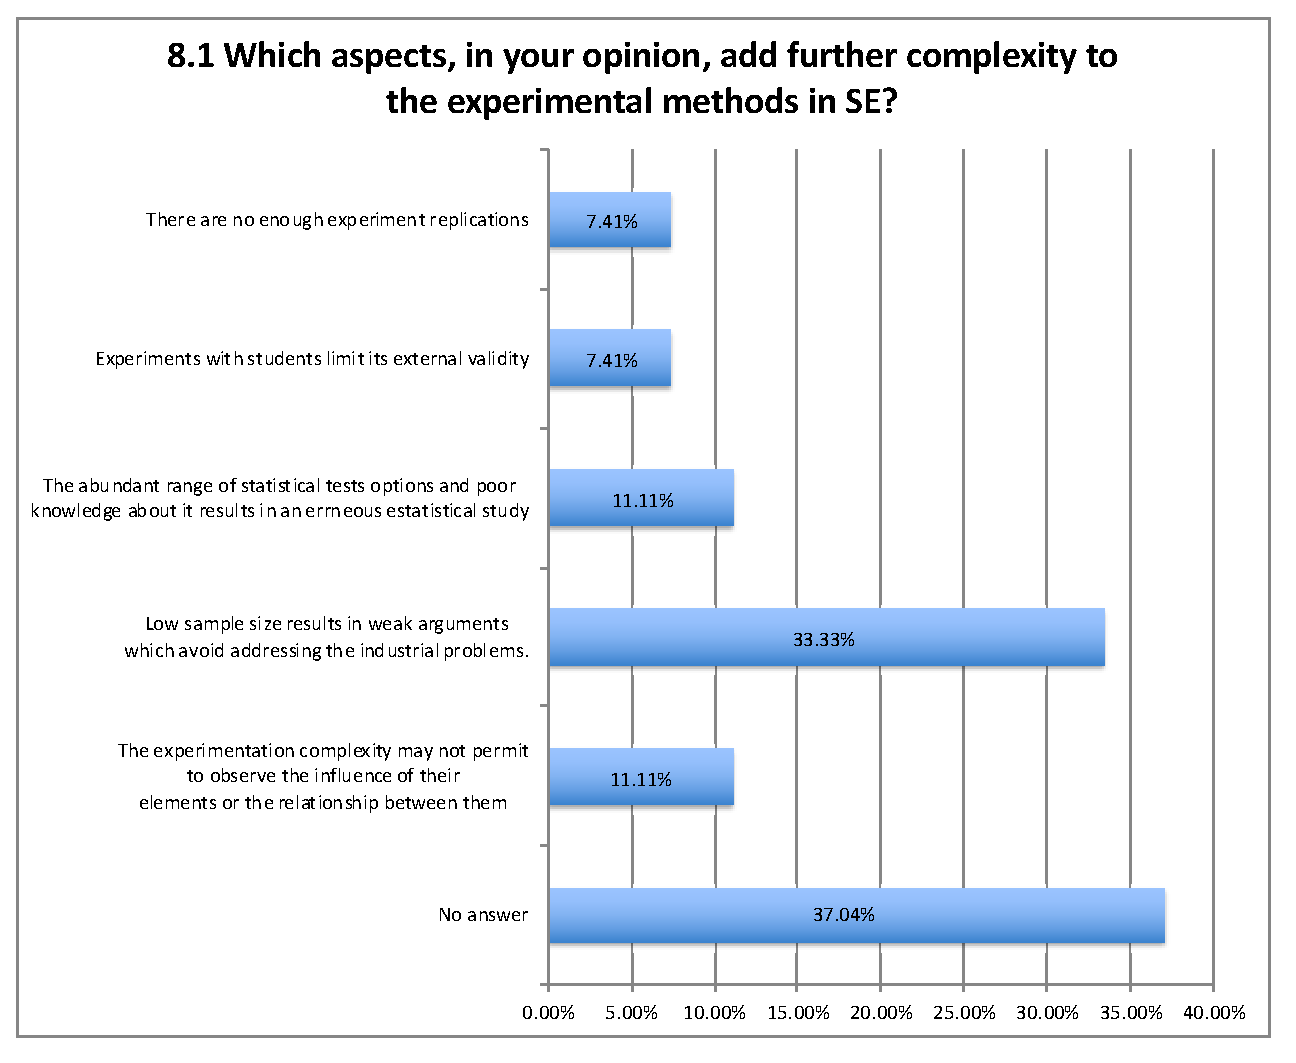
\includegraphics[width=12cm]{Images/Factors-Influencing-Complexity-ESE}
	\caption{Factors influencing the complexity of experimentation in SE}
	\label{fig-Factors-Influencing-Complexity-ESE}
\end{figure*}

As� mismo, un 11\% de los investigadores piensan que {\color{green}(SC11)} \ul{the experimentation complexity may not permit to observe the influence of their elements or the relationship between them}; mientras que otros investigadores son m�s espec�ficos y le atribuyen la complejidad de la experimentaci�n a que {\color{green}(SC12)} \ul{there are no enough experiment replications} (7.41\%) y a que los {\color{green}(SC13)} \ul{experiments with students limit its external validity} (7.41\%).

Por otra parte, otro problema remarcado en este estudio es el referido a la dificultad en la gesti�n de los datos. Un 14.81\% considera que {\color{green}(SC14)} \ul{el manejo y el an�lisis de los datos experimentales son complejos, lo que podr�a deberse en parte a las distintas maneras que tienen los investigadores para gestionarlos}: Un 66.67\% afirma que utilizan hojas de calculo, un 25\% repositorios de datos relacionales y un 44\% formatos propietarios. Por otra parte, un 7.41\% de los encuestados hace �nfasis en la limitada compartici�n de datos que existe, lo que es corroborado por mas de un 10\% de investigadores que consideran que {\color{green}(SC15)} \ul{la agregaci�n de datos entre replicaciones es compleja, quiz� en parte porque no existe un soporte adecuado para las replicaciones y la existencia del conocimiento t�cito}.

\begin{tcolorbox}

los aspectos que consideramos como problem�ticos en torno a la SE experimentation fueron corroborados en gran medida por los encuestados, e incluso se obtuvieron importantes recomendaciones a ser consideradas (ver Fig. \ref{fig-recommendations-improve-SE-experimentation}):

\begin{itemize}
  \item To have a common empirical source of knowledge
  \item To use simple guidelines to report findings
  \item To formalize the process
  \item To formalize the terminology
  \item To apply statistical test depending on experiment design
  \item To have a set of selected experimental subjects
  \item To receive quality formal courses
\end{itemize}

\end{tcolorbox}

\begin{figure*}[htbp!]
	\centering
	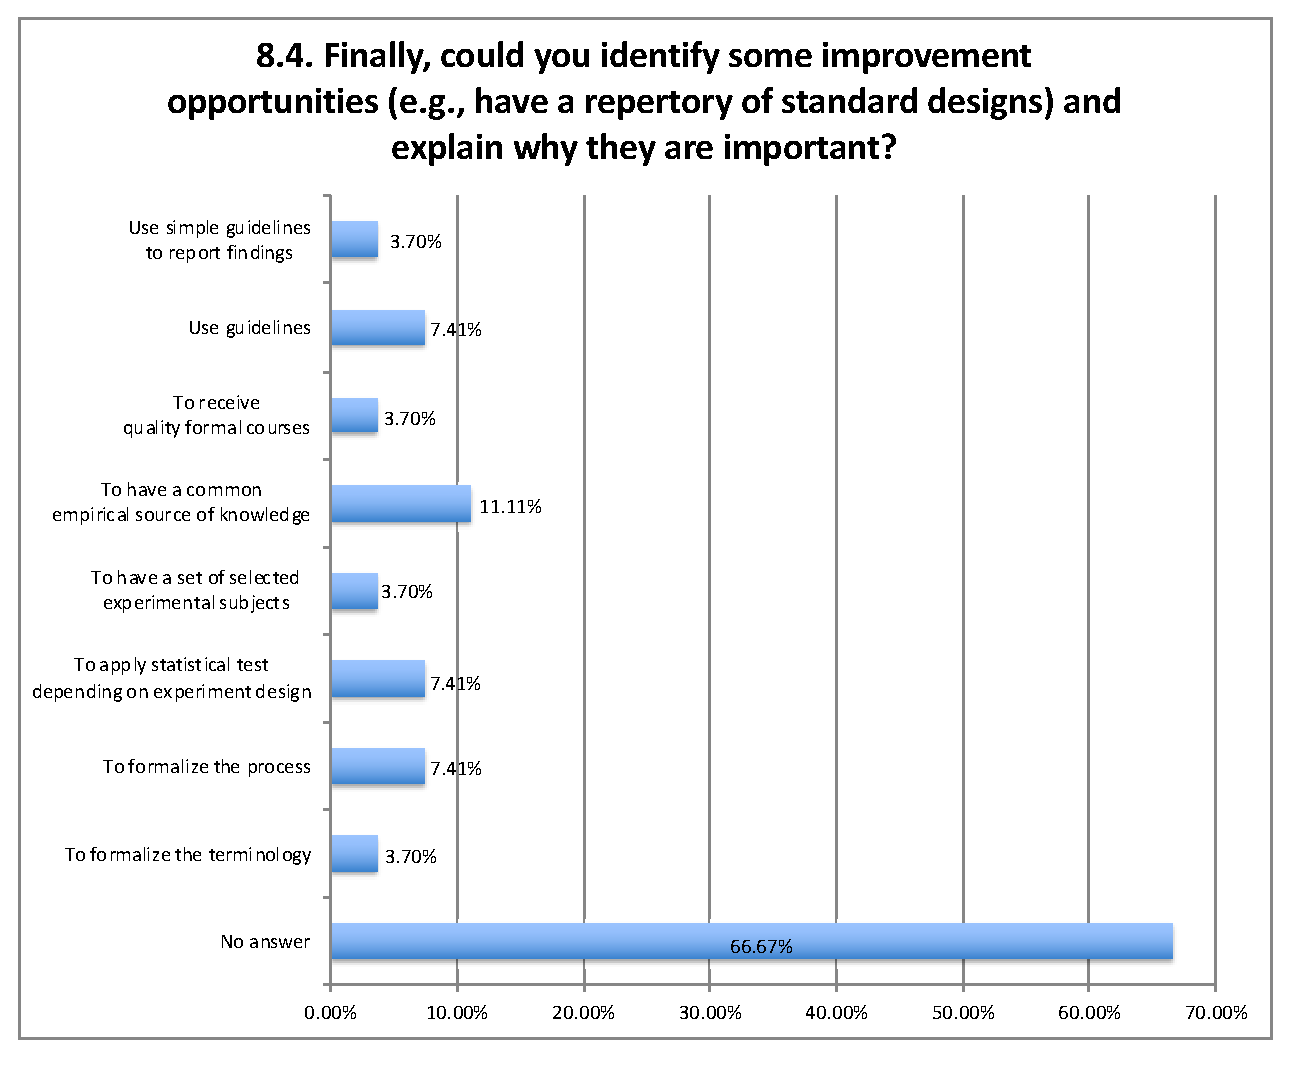
\includegraphics[width=12cm]{Images/Recommendations-Improve-SE-Experimentation}
	\caption{Recommendations to Improve the Experimentation in SE}
	\label{fig-recommendations-improve-SE-experimentation}
\end{figure*}

%%
%% References

\bibliographystyle{ACM-Reference-Format}
\bibliography{Biblio-Experimental-Process-SE} % name your BibTeX data base

%%
%% ACKs

\begin{acks}
  \odnote{A\~nadir ACKS}
\end{acks}

%%
%% Appendices

\clearpage
\onecolumn

\appendix

\section{Conceptual models generated during the ethnographical research}\label{sec:annex_models}

Las figuras contienen t�rminos en Espa�ol, idioma en que se realiz� la investigaci�n. Hemos preferido no traducir las figuras para asegurar la trazabilidad entre en art�culo y la raw data, disponible en \url{}\odnote{RODRIGO: Indicar ubicaci�n de la raw data}.

\begin{figure*}[htbp!]
	\centering
	\captionsetup{justification=centering}
	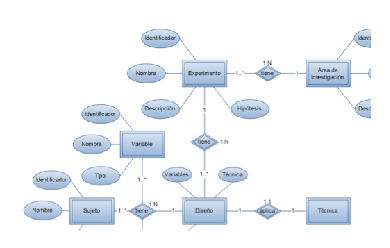
\includegraphics[width=\textwidth]{images/Producto-Intermedio-Revision-Lit}
	\caption{Modelo conceptual preliminar resultado del an�lisis de la literatura relevante.}
	\label{fig-conceptos-preliminar}
	\odnote{RODRIGO: He movido la figura a un anexo. Que se vea entera. D�jala en Espa�ol, ya que es posible que haya que haya que enlazar a ese ap�ndice el resto del row data de la tesis}
\end{figure*}

\begin{figure*}[htbp!]
	\centering
	
\includegraphics[width=5in]{images/Producto-Final-Revision-Lit}
	\caption{Modelo conceptual resultado del an�lisis de los materiales experimentales.}
	\label{fig-conceptos-final-revision-fuentes}\odnote{RODRIGO: Pon el modelo completo.}
\end{figure*}

\begin{figure*}[htbp!]
	\centering
	\includegraphics[width=5in]{images/Producto-Final-Observacion-Par}
	\caption{Modelo conceptual resultado de la observaci�n participativa.}
	\label{fig-conceptos-final-observacion-participativa}\odnote{RODRIGO: Hay que crear esta figura.}
\end{figure*}

\begin{figure*}[htbp!]
	\centering
	\includegraphics[width=5in]{images/Model}
	\caption{Modelo conceptual resultado de las entrevistas semi-estructuradas.}
	\label{fig-modelo-exp}\odnote{RODRIGO: Hay que crear esta figura.}
\end{figure*}

\begin{figure}[htbp!]
	\centering
	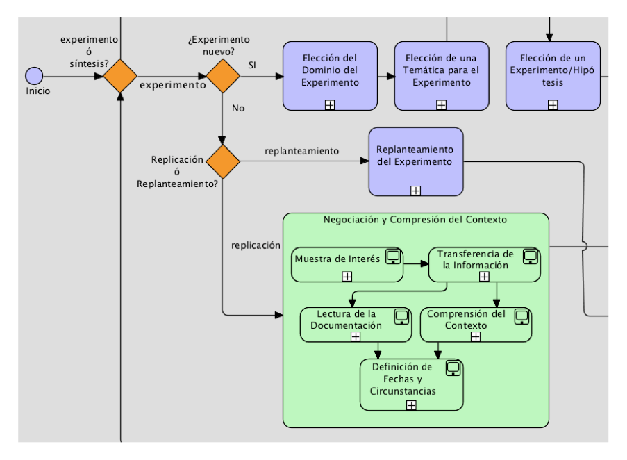
\includegraphics[width=3.2in]{images/Proccess}
	\caption{Diagrama de procesos resultado de las entrevistas semi-estructuradas.}
	\label{fig-proceso-exp}\odnote{RODRIGO: Pon el modelo completo.}\odnote{RODRIGO: No se produjo una evoluci�n de los modelos conceptuales?}
\end{figure}


%=========================

\end{document}
\endinput

